%  LaTeX support: latex@mdpi.com
%  For support, please attach all files needed for compiling as well as the log file, and specify your operating system, LaTeX version, and LaTeX editor.

%=================================================================
\documentclass[entropy,article,submit,moreauthors,LaTeX and dvi2pdf]{Definitions/mdpi}

% For posting an early version of this manuscript as a preprint, you may use "preprints" as the journal and change "submit" to "accept". The document class line would be, e.g., \documentclass[preprints,article,accept,moreauthors,pdftex]{mdpi}. This is especially recommended for submission to arXiv, where line numbers should be removed before posting. For preprints.org, the editorial staff will make this change immediately prior to posting.

%--------------------
% Class Options:
%--------------------
%----------
% journal
%----------
% Choose between the following MDPI journals:
% acoustics, actuators, addictions, admsci, adolescents, aerospace, agriculture, agriengineering, agronomy, ai, algorithms, allergies, analytica, animals, antibiotics, antibodies, antioxidants, appliedchem, applmech, applmicrobiol, applnano, applsci, arts, asi, atmosphere, atoms, audiolres, automation, axioms, batteries, bdcc, behavsci, beverages, biochem, bioengineering, biologics, biology, biomechanics, biomedicines, biomedinformatics, biomimetics, biomolecules, biophysica, biosensors, biotech, birds, bloods, brainsci, buildings, businesses, cancers, carbon, cardiogenetics, catalysts, cells, ceramics, challenges, chemengineering, chemistry, chemosensors, chemproc, children, civileng, cleantechnol, climate, clinpract, clockssleep, cmd, coatings, colloids, compounds, computation, computers, condensedmatter, conservation, constrmater, cosmetics, crops, cryptography, crystals, curroncol, cyber, dairy, data, dentistry, dermato, dermatopathology, designs, diabetology, diagnostics, digital, disabilities, diseases, diversity, dna, drones, dynamics, earth, ebj, ecologies, econometrics, economies, education, ejihpe, electricity, electrochem, electronicmat, electronics, encyclopedia, endocrines, energies, eng, engproc, entropy, environments, environsciproc, epidemiologia, epigenomes, fermentation, fibers, fire, fishes, fluids, foods, forecasting, forensicsci, forests, fractalfract, fuels, futureinternet, futuretransp, futurepharmacol, futurephys, galaxies, games, gases, gastroent, gastrointestdisord, gels, genealogy, genes, geographies, geohazards, geomatics, geosciences, geotechnics, geriatrics, hazardousmatters, healthcare, hearts, hemato, heritage, highthroughput, histories, horticulturae, humanities, hydrogen, hydrology, hygiene, idr, ijerph, ijfs, ijgi, ijms, ijns, ijtm, ijtpp, immuno, informatics, information, infrastructures, inorganics, insects, instruments, inventions, iot, j, jcdd, jcm, jcp, jcs, jdb, jfb, jfmk, jimaging, jintelligence, jlpea, jmmp, jmp, jmse, jne, jnt, jof, joitmc, jor, journalmedia, jox, jpm, jrfm, jsan, jtaer, jzbg, kidney, land, languages, laws, life, liquids, literature, livers, logistics, lubricants, machines, macromol, magnetism, magnetochemistry, make, marinedrugs, materials, materproc, mathematics, mca, measurements, medicina, medicines, medsci, membranes, metabolites, metals, metrology, micro, microarrays, microbiolres, micromachines, microorganisms, minerals, mining, modelling, molbank, molecules, mps, mti, nanoenergyadv, nanomanufacturing, nanomaterials, ncrna, network, neuroglia, neurolint, neurosci, nitrogen, notspecified, nri, nursrep, nutrients, obesities, oceans, ohbm, onco, oncopathology, optics, oral, organics, osteology, oxygen, parasites, parasitologia, particles, pathogens, pathophysiology, pediatrrep, pharmaceuticals, pharmaceutics, pharmacy, philosophies, photochem, photonics, physchem, physics, physiolsci, plants, plasma, pollutants, polymers, polysaccharides, proceedings, processes, prosthesis, proteomes, psych, psychiatryint, publications, quantumrep, quaternary, qubs, radiation, reactions, recycling, regeneration, religions, remotesensing, reports, reprodmed, resources, risks, robotics, safety, sci, scipharm, sensors, separations, sexes, signals, sinusitis, smartcities, sna, societies, socsci, soilsystems, solids, sports, standards, stats, stresses, surfaces, surgeries, suschem, sustainability, symmetry, systems, taxonomy, technologies, telecom, textiles, thermo, tourismhosp, toxics, toxins, transplantology, traumas, tropicalmed, universe, urbansci, uro, vaccines, vehicles, vetsci, vibration, viruses, vision, water, wevj, women, world

%---------
% article
%---------
% The default type of manuscript is "article", but can be replaced by:
% abstract, addendum, article, book, bookreview, briefreport, casereport, comment, commentary, communication, conferenceproceedings, correction, conferencereport, entry, expressionofconcern, extendedabstract, datadescriptor, editorial, essay, erratum, hypothesis, interestingimage, obituary, opinion, projectreport, reply, retraction, review, perspective, protocol, shortnote, studyprotocol, systematicreview, supfile, technicalnote, viewpoint, guidelines, registeredreport, tutorial
% supfile = supplementary materials

%----------
% submit
%----------
% The class option "submit" will be changed to "accept" by the Editorial Office when the paper is accepted. This will only make changes to the frontpage (e.g., the logo of the journal will get visible), the headings, and the copyright information. Also, line numbering will be removed. Journal info and pagination for accepted papers will also be assigned by the Editorial Office.

%------------------
% moreauthors
%------------------
% If there is only one author the class option oneauthor should be used. Otherwise use the class option moreauthors.

%---------
% pdftex
%---------
% The option pdftex is for use with pdfLaTeX. If eps figures are used, remove the option pdftex and use LaTeX and dvi2pdf.

%=================================================================
% MDPI internal commands
\firstpage{1}
\makeatletter
\setcounter{page}{\@firstpage}
\makeatother
\pubvolume{1}
\issuenum{1}
\articlenumber{0}
\pubyear{2021}
\copyrightyear{2020}
%\externaleditor{Academic Editor: Firstname Lastname} % For journal Automation, please change Academic Editor to "Communicated by"
\datereceived{}
\dateaccepted{}
\datepublished{}
\hreflink{https://doi.org/} % If needed use \linebreak
%------------------------------------------------------------------
% The following line should be uncommented if the LaTeX file is uploaded to arXiv.org
%\pdfoutput=1

%=================================================================
% Add packages and commands here. The following packages are loaded in our class file: fontenc, inputenc, calc, indentfirst, fancyhdr, graphicx, epstopdf, lastpage, ifthen, lineno, float, amsmath, setspace, enumitem, mathpazo, booktabs, titlesec, etoolbox, tabto, xcolor, soul, multirow, microtype, tikz, totcount, changepage, paracol, attrib, upgreek, cleveref, amsthm, hyphenat, natbib, hyperref, footmisc, url, geometry, newfloat, caption
\usepackage{siunitx}
\usepackage{subfigure}
\usepackage{longtable}
\usepackage{footnote}
% \usepackage{multirow}
% \usepackage{indentfirst}
\usepackage{tabu}
%=================================================================
%% Please use the following mathematics environments: Theorem, Lemma, Corollary, Proposition, Characterization, Property, Problem, Example, ExamplesandDefinitions, Hypothesis, Remark, Definition, Notation, Assumption
%% For proofs, please use the proof environment (the amsthm package is loaded by the MDPI class).

%=================================================================
% Full title of the paper (Capitalized)
\Title{Driving Risk Assessment Using Near-miss Events Based on Panel Poisson Regression and Panel Negative Binomial Regression}

% MDPI internal command: Title for citation in the left column
\TitleCitation{Driving Risk Assessment Using Near-miss Events Based on Panel Poisson Regression and Panel Negative Binomial Regression}

% Author Orchid ID: enter ID or remove command
\newcommand{\orcidauthorA}{0000-0001-5654-5104} % Add \orcidA{} behind the author's name
\newcommand{\orcidauthorB}{0000-0002-2644-6268} % Add \orcidB{} behind the author's name
\newcommand{\orcidauthorC}{0000-0002-8318-0603} % Add \orcidC{} behind the author's name

% Authors, for the paper (add full first names)
\Author{Shuai Sun $^{1,\dagger}$\orcidA{}, Jun Bi$^{1,}$*, Montserrat Guillen $^{2,}$*\orcidB{} and Ana M. Pérez-Marín $^{2}$\orcidC{}}

% MDPI internal command: Authors, for metadata in PDF
\AuthorNames{Shuai Sun, Jun Bi, Montserrat Guillen and Ana M. Pérez-Marín}

% MDPI internal command: Authors, for citation in the left column
\AuthorCitation{Shuai, S.; Jun, B.; Guillen, M.; Pérez-Marín, A. M.}
% If this is a Chicago style journal: Lastname, Firstname, Firstname Lastname, and Firstname Lastname.

% Affiliations / Addresses (Add [1] after \address if there is only one affiliation.)
\address{%
$^{1}$ \quad Key Laboratory of Transport Industry of Big Data Application Technologies for Comprehensive Transport, School of Traffic and Transportation, Beijing Jiaotong University, China; sunshuai@bjtu.edu.cn(S.S.)\\
$^{2}$ \quad Dept. of Econometrics, Riskcenter-IREA, Universitat de Barcelona, Spain; mguillen@ub.edu (M.G.); amperez@ub.edu (A.M.P.-M.)}

% Contact information of the corresponding author
\corres{Correspondence: bilinghc@163.com(J.B.), mguillen@ub.edu(M.G.); Tel.: +86-13488812321(J.B.), +34-934037039(M.G.)}

% Current address and/or shared authorship
\firstnote{Current address: Dept. of Econometrics, Riskcenter-IREA, Universitat de Barcelona, Spain}
% \secondnote{These authors contributed equally to this work.}
% The commands \thirdnote{} till \eighthnote{} are available for further notes

%\simplesumm{} % Simple summary

%\conference{} % An extended version of a conference paper

% Abstract (Do not insert blank lines, i.e. \\)
\abstract{This study proposes a method to identify and evaluate driving risk as the primary step to calculate premiums in the newly emerging context of usage-based insurance. Telematics data obtained from the Internet of vehicles contains a large number of near-miss events, which can be regarded as an alternative to modeling claims or accidents, to estimate a driving risk score for each vehicle.  Poisson regression and Negative binomial regression are applied to a summary data set with one record per vehicle and to a panel data set of daily vehicle data containing near-miss events; i.e. counts of excess speed, high speed brake, harsh acceleration or deceleration, and additional driving behavior parameters not including accidents. Negative binomial regression performs better than Poisson regression. Vehicles are classified with a driving risk score computed from individual effects of the panel model. This study provides a research basis for actuarial insurance premium calculations even if no accident information is available and enables precise supervision of dangerous driving behaviors based on driving risk scores.}

% Keywords
\keyword{driving risk assessment; usage-based insurance (UBI); driving risk score; telematics; near-miss event; driving behavior; panel data analysis; count data model; econometrics}

% The fields PACS, MSC, and JEL may be left empty or commented out if not applicable
%\PACS{J0101}
%\MSC{}
%\JEL{}

%%%%%%%%%%%%%%%%%%%%%%%%%%%%%%%%%%%%%%%%%%
% Only for the journal Diversity
%\LSID{\url{http://}}

%%%%%%%%%%%%%%%%%%%%%%%%%%%%%%%%%%%%%%%%%%
% Only for the journal Applied Sciences:
%\featuredapplication{Authors are encouraged to provide a concise description of the specific application or a potential application of the work. This section is not mandatory.}
%%%%%%%%%%%%%%%%%%%%%%%%%%%%%%%%%%%%%%%%%%

%%%%%%%%%%%%%%%%%%%%%%%%%%%%%%%%%%%%%%%%%%
% Only for the journal Data:
%\dataset{DOI number or link to the deposited data set in cases where the data set is published or set to be published separately. If the data set is submitted and will be published as a supplement to this paper in the journal Data, this field will be filled by the editors of the journal. In this case, please make sure to submit the data set as a supplement when entering your manuscript into our manuscript editorial system.}

%\datasetlicense{license under which the data set is made available (CC0, CC-BY, CC-BY-SA, CC-BY-NC, etc.)}

%%%%%%%%%%%%%%%%%%%%%%%%%%%%%%%%%%%%%%%%%%
% Only for the journal Toxins
%\keycontribution{The breakthroughs or highlights of the manuscript. Authors can write one or two sentences to describe the most important part of the paper.}

%%%%%%%%%%%%%%%%%%%%%%%%%%%%%%%%%%%%%%%%%%
% Only for the journal Encyclopedia
%\encyclopediadef{Instead of the abstract}
%\entrylink{The Link to this entry published on the encyclopedia platform.}
%%%%%%%%%%%%%%%%%%%%%%%%%%%%%%%%%%%%%%%%%%

\begin{document}
%%%%%%%%%%%%%%%%%%%%%%%%%%%%%%%%%%%%%%%%%%
\section{Introduction}

Near-miss events are incidents that denote the existence of danger, even if no accident occurs. Reporting of near-miss event is an established error reduction technique that has been used by many industries to manage risk and reduce accidents. In the auto insurance industry, insurers traditionally calculate premiums by analyzing the claims the insured policy holders reported in the past and reward with discounts those drivers that do not report accidents. However, this may be a rather incorrect approach to assess accident risk, when the insured has suffered accidents but has not claimed to avoid loosing a discount. Fortunately, the advent of internet of vehicles (IoV) has given an improved solution to this problem, using near-miss events to identify driving risk. Near-miss events ultimately provide information that can lead to actuarial premium calculations in the auto insurance industry\cite{guillen2020can}.

This study purposes to explore how to evaluate driving risks and score drivers in the short term without claims and accidents, but based on information on near-miss counts in a short period of time. Dealing with the absence of claims combined with a short period of observation of the drivers using telematics sensors is one of the main novelties of our approach. The model obtained in this study has important significance for driving risk identification. Not only can the model reflect risk factors that influence each near-miss event, but the coefficients can also help us evaluate drivers' risks and fixed-effects panel count data models can be used to rank drivers according to their individual effects. The modeling method and results are valuable for insurance companies to develop usage-based insurance (UBI) to personalize premiums. In addition, they are also interesting for traffic regulatory authorities to promote safe driving and prevent accidents.

Near-miss events are incidents that need to be defined and extracted from the original raw data files for further processing and analysis. Because the original telematics data in this study does not contain claims or accidents, the extraction of near-miss events that are highly relevant to identify driving patterns is critical. This study was carried out both on a per driver summary data set and on a panel data set where each driver has a daily summary. Our data contain counts of the four near-miss events in our study. Here, over speed, high speed braking, harsh acceleration and harsh deceleration, have been defined based on actual driving conditions and local laws and regulations. Some other near-miss events, e.g. sharp turning, dangerous lane changing and unexpected maneuver were not included in this study due to the dimension and precision limitations of the original data set. Since the extracted frequency of near-miss events is an unbounded non-negative integer, Poisson regression and Negative binomial regression are suitable for modelization.

Poisson regression, Negative binomial regression, Zero-inflated Poisson regression and Zero-inflated Negative binomial regression were respectively applied to the summary data set. Average speed, brake times, accelerator pedal position, engine fuel rate etc., were selected as independent variables\cite{sun2020assessing}. In particular, either mileage or fuel consumption could be chosen as exposure variable to offset the model. In order to have a clear understanding of risky factors of different near-miss events, each near-miss event was individually used as a dependent variable. However, no matter which one was selected as the dependent variable, Negative binomial regression provide the best fit in the summary data in this study.

Negative binomial regression also performed better than Poisson regression on the panel data sets. Individual effects and time effects were estimated using panel Poisson regression and panel Negative binomial regression on our short panel data set of 6 days in length. The regression results not only confirmed the existence of individual effects and time effects but allowed the driving risk of each vehicle to be ranked. Then, according to the individual effects converted into scores, the driving risk level of vehicles could be classified, providing an important reference for further accurate calculation of premiums.

The rest of this article is organized as follows. The development of UBI and previous efforts on driving risk assessment are summarized in Section 2. Section 3 describes the data and introduces the key parameters used in modeling. Section 4 presents the model expression of Poisson regression and Negative binomial regression in this study. Negative binomial regression results on summary data set and panel data set are reported and analysed in Section 5. The results are discussed and the conclusions are presented in Section 6.
%%%%%%%%%%%%%%%%%%%%%%%%%%%%%%%%%%%%%%%%%%

\section{Literature Review}
The auto insurance industry has never stopped pursuing new ways to calculate more accurate actuarial premiums. However, traditional auto insurance business has been limited by the difficulty of obtaining information on policy holders, so classical ratemaking uses simple information of drivers (age and gender), vehicles (type of car, model and brand) and driving sections\cite{litman2007distance}. With the continuous progress of information technology, a new type of insurance business, UBI, based on multi-source data and personalized premium calculation is becoming the mainstream. Pay-as-you-drive (PAYD) mode of charging premiums depends on the driving mileage or fuel consumption and is based on the premise that mileage or fuel consumption correlatives with the probability of suffering an accident\cite{tselentis2016innovative}. Then, PAYD has evolved into a newer scheme, called the pay-how-you-drive (PHYD) ratemaking mode, which is based on multiple sources of data including driving behavior data\cite{paefgen2013evaluation}. After the development of 5G communication technology, it may be possible to implement an even more sophisticated monitoring and pricing strategy known as the manage-how-you-drive (MHYD) principle, i.e. real-time calculation of premiums based on multi-source data and providing real-time information to drivers to restrain bad driving behavior\cite{litman2007distance,tselentis2017innovative}. However, due to various reasons such as technological, regulatory and other issues regarding privacy\cite{troncoso2010pripayd}, there is still no mature PHYD product on the market at present\cite{pesantez2019predicting,guillen2019use}. In terms of MHYD, driving risk needs to be further studied to produce products that are more suitable for meeting the demand\cite{sun2020assessing}.

Traffic accidents all over the world cause a large number of casualties every year, and high risk driving is one of the main factors that cause traffic accidents\cite{litman2007distance}. Therefore, the research on driving risk has been a hot topic in recent decades. Fundamentally, simulation experiments have beeb designed in the laboratory setting to identify driving risk factors\cite{de2013analysis,siordia2014subjective,charlton2014s,peng2018intelligent}. Further,real vehicle experiments on real road environments have been conducted to evaluate driving risk\cite{wang2015driving,yan2016hazardous,liao2018cross,jiang2019real,yan2019driving}. In addition, questionnaire surveys for driving risk assessment have also been studied \cite{lu2013focusing,wang2020driving}. In fact, the naturalistic type of driving data collected by the Internet of vehicles or smart phones, telematics data, can effectively reduce the influence of subjective factors and unreasonable assumptions in producing effective risk mitigating actions\cite{handel2014insurance,joubert2016combining,verbelen2018unravelling,ma2018use,jiang2020drivers}.

In the research of driving risk assessment in the auto insurance industry, machine learning and generalized linear models coexist. With its strong ability to process big data efficiently, machine learning is increasingly entering explored the auto insurance business. Logistic regression\cite{jin2018latent}, cluster analysis\cite{carfora2019pay}, decision tree\cite{paefgen2013evaluation}, support vector machine\cite{burton2016driver}, neural network\cite{baecke2017value} and other machine learning models\cite{guelman2012gradient,bian2018good,jafarnejad2017towards} have been widely studied in the field of driving risk assessment, and the results also show that machine learning is a powerful tool \cite{paefgen2014multivariate}. However, since most machine learning procedures as black box algorithms do not have good interpretability, they cannot completely replace the conventional generalized linear models implemented for decades in the auto insurance industry\cite{pesantez2019predicting}.

Conventional generalized linear models pay attention to the correlation between influencing factors and claims or accidents in frequency and severty models\cite{boucher2013pay,verbelen2018unravelling,ma2018use,guillen2019use}. But the study of near-miss events even when there is a lack of information on claims and accidents should not be ignored\cite{wang2015driving,guillen2020can}, on the contrary, since near-miss events are more frequent than accidents and they are positively associated with them, near-miss events can be considered good alternatives for risk modeling for driving risk assessment.
%%%%%%%%%%%%%%%%%%%%%%%%%%%%%%%%%%%%%%%%%%
\section{Data Description}
The telematics data used in this study is collected from an IoV information service provider in China. The original data set contains 182 data files representing sensor data for 182 vehicles observed from July 3, 2018 to July 8, 2018\cite{sun2020assessing}. Each data file contains 62 different measurements, but after data processing\cite{sun2019cleaning}, less than one-third of them could be retained due to recording errors and inconsistencies. The original data were transformed for modeling into summary data set, with  information on each driver (see details in Table~\ref{summary}).

\begin{specialtable}[htbp]
\widetable
\caption{Descriptive statistics of summary data set.}
\label{summary}
\resizebox{\textwidth}{!}{
\begin{tabular}{cccccccc}
\toprule
Variable                & Mean  & Standard Deviation & Minimum & Median & Maximum & Defination&  \\
\midrule
overspeed                & 19.19 & 45.37              & 0  & 0     & 330     & Cumulative times of driving speed greater than 100km/h                        &  \\
highspeedbrake           & 44.23 & 108.3              & 0  & 4     & 942     & Cumulative times of braking when the driving speed is greater than 90km/h    &  \\
harshacceleration        & 139.0 & 134.7              & 0  & 101     & 899     & Cumulative times of the acceleration is greater than $6m/s^2$ &  \\
harshdeceleration        & 141.9 & 137.8              & 1  & 105     & 913     & Cumulative times of the acceleration is less than $6m/s^2$    &  \\
kilo                     & 2,223 & 1,674              & 3.73 & 1832.175  & 7,164   & Cumulative driving distance (km)                                             &  \\
fuel                     & 621.7 & 470.9              & 10.25 & 487.295   & 2,018   & Cumulative fuel consumption (L)                                              &  \\
brakes                   & 1,588 & 1,426              & 6 & 1138.5      & 9,243   & Cumulative number of brakes                                                  &  \\
range                    & 5.201 & 5.021              & 0.027 &3.399  & 26.78   & Range of driving (geographical units)                                        &  \\
speed                    & 36.88 & 16.37              & 0.297 & 36.657   & 67.84   & Mean of speed (km/h)                                                         &  \\
rpm                      & 1,028 & 188.3              & 233.1 &1009.301   & 1,620   & Mean of revolutions per minute (r/min)                                       &  \\
acceleratorpedalposition & 21.05 & 7.110              & 0.187 & 21.26   & 39.29   & Mean of acceleration pedal position (\%)                                     &  \\
enginefuelrate           & 11.52 & 4.464              & 1.868 &11.203   & 22.01   & Mean of engine fuel rate (\%)   & \\
\bottomrule
\footnotesize{$^a$ The number of each parameter is 182.}
\end{tabular}}
\end{specialtable}
\begin{paracol}{2}
\linenumbers
\switchcolumn
In particular, $overspeed$, $highspeedbrake$, $harshacceleration$ and $harshdeceleration$ are individually filtered by combining the rules of traffic law and driving code. Firstly, previous studies have confirmed that over speed is a dangerous driving behavior that is likely to cause traffic accidents\cite{litman2007distance}. And China's traffic safety regulations stipulate a maximum speed for the each type of vehicles on all types of roads. The maximum speed limit of the vehicles in this study is 90 km/h, and it is not illegal to exceed the speed limit by less than ten percent. Therefore, 100 km/h is taken as the threshold value of the overspeed near-miss event. Secondly, if the emergency braking of a car running at a high speed is operated improperly or subjected to lateral force, it is prone to side-slip or even cartwheel, thus high-speed (>90km/h) braking is a risky near-miss event worthy of study. Thirdly, both harsh acceleration and harsh deceleration are near-miss events that need to be avoided in terms of driving safety and fuel economy. Based on the previous research experience\cite{gao2019evaluation,guillen2020can} and the filter analysis of the extreme values of this data set by box graph method, $6m/s^2$ is determined as the filtering threshold value of harsh acceleration and harsh deceleration. It can be seen from Figure~\ref{frequency} that near-miss events are all non-negative integers. Combined with the relationship between expectation and variance shown in Table~\ref{summary}, the four near-miss events are suitable as dependent variables of a Poisson regression or a Negative binomial regression.
\end{paracol}
\begin{figure}[htbp]
	\widefigure
	\subfigure[]{
		\begin{minipage}[t]{0.45\textwidth}
		\centering
		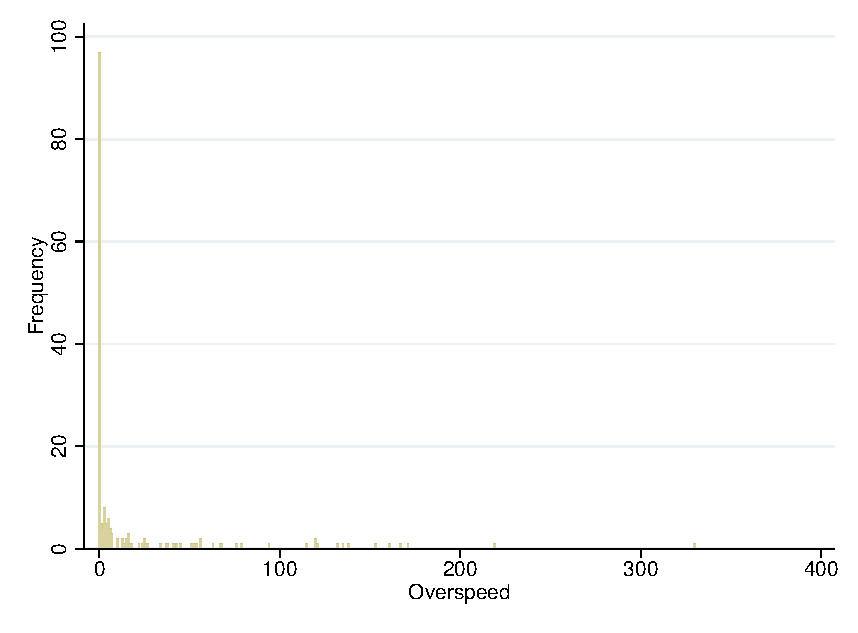
\includegraphics[width=1\textwidth]{Figure/Overspeed.eps}
		\end{minipage}
		\label{frequency_a}
	}
    \subfigure[]{
    	\begin{minipage}[t]{0.45\textwidth}
    	\centering
   		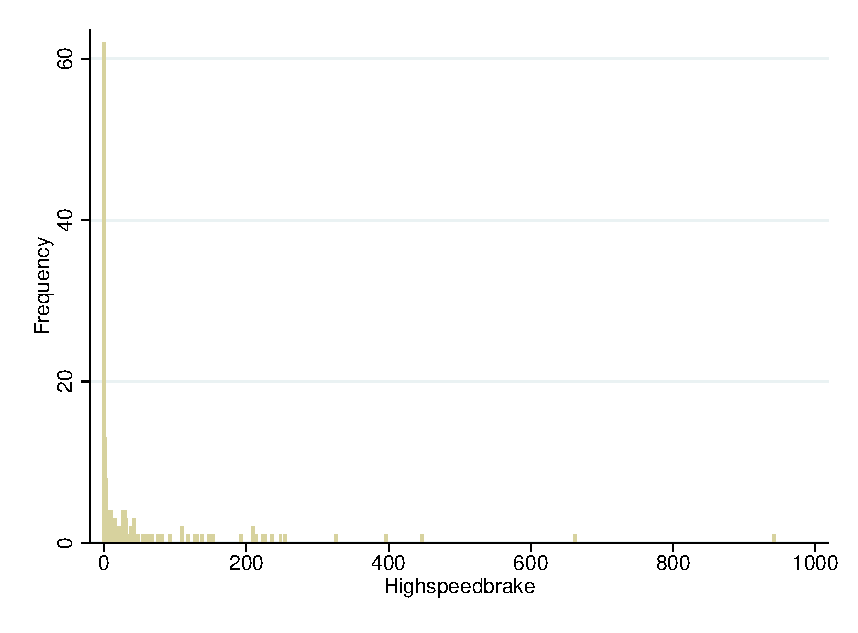
\includegraphics[width=1\textwidth]{Figure/Highspeedbrake.eps}
    	\end{minipage}
		\label{frequency_b}
    	}
	\\
	\subfigure[]{
		\begin{minipage}[t]{0.45\textwidth}
		\centering
		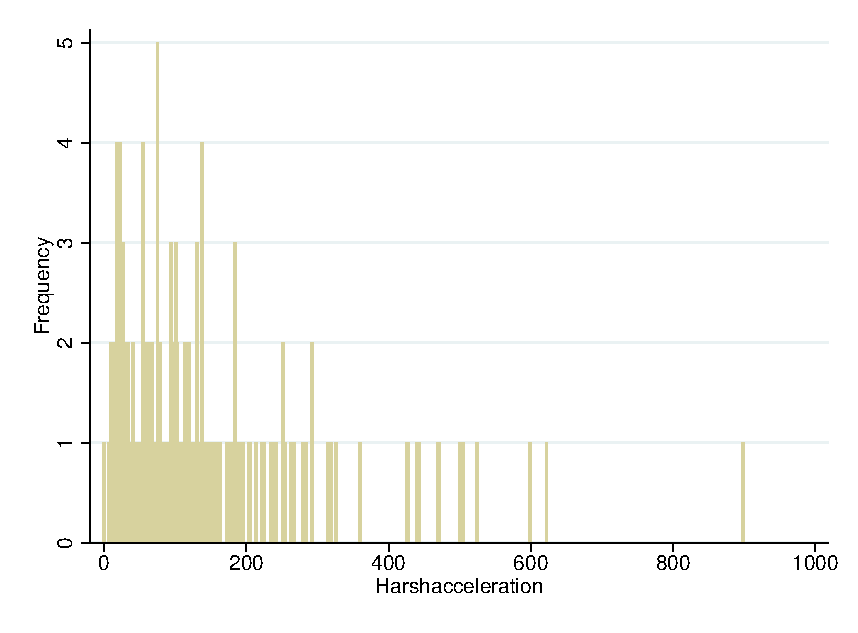
\includegraphics[width=1\textwidth]{Figure/Harshacceleration.eps}
		\end{minipage}
		\label{frequency_c}
	}
    \subfigure[]{
    	\begin{minipage}[t]{0.45\textwidth}
    	\centering
		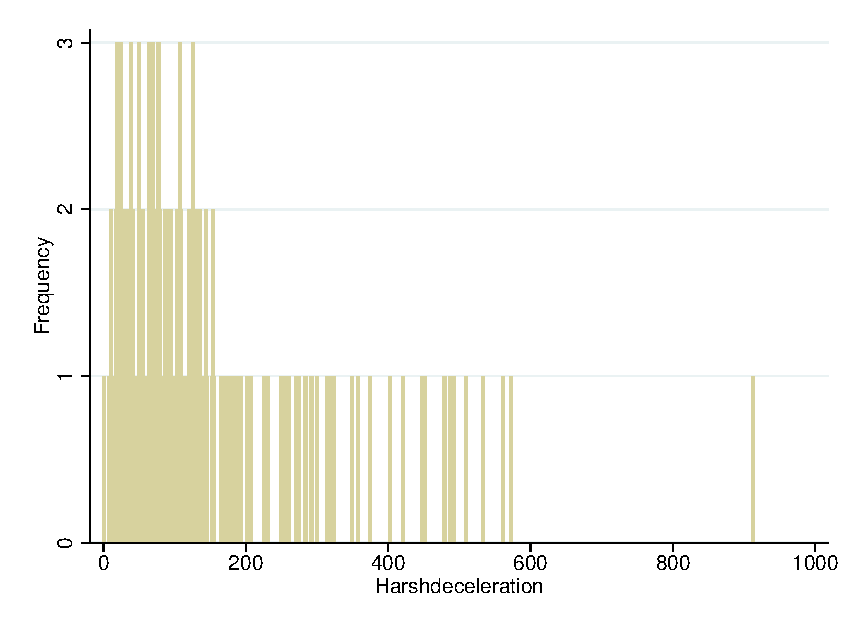
\includegraphics[width=1\textwidth]{Figure/Harshdeceleration.eps}
    	\end{minipage}
		\label{frequency_d}
    	}
	\caption{Histogram of frequency distribution of four near-miss events: (a)Over speed;(b)High speed brake;(c)Harsh acceleration;(d)Harsh deceleration.}
	\label{frequency}
\end{figure}
\begin{paracol}{2}
\linenumbers
\switchcolumn
The panel data set has one summary per day for each driver. The statistics of panel data set are shown in the Table \ref{panel}.
\end{paracol}
\begin{specialtable}[htbp]
\widetable
\caption{Descriptive statistics of a panel data set for 182 drivers observed over six days (total cases 1092).}
\label{panel}
\begin{tabular}{cccccccc}
\toprule
Variable               & N     & Mean  & Standard Deviation & Minimum & Median & Maximum \\
\midrule
overspeed                & 1,092 & 3.199 & 14.37              & 0   &0    & 315     \\
highspeedbrake           & 1,092 & 7.435 & 21.74              & 0   &0    & 215     \\
harshacceleration        & 1,092 & 23.37 & 29.78              & 0   &14    & 223     \\
harshdeceleration        & 1,092 & 23.86 & 30.16              & 0   &13.5    & 233     \\
kilo                     & 1,092 & 372.6 & 373.2              & 0   &263.24    & 1,739   \\
fuel                     & 1,092 & 104.1 & 105.7              & 0   &72.15    & 565.8   \\
brakes                   & 1,092 & 264.7 & 291.0              & 0   &178    & 1,940   \\
range                    & 1,092 & 2.406 & 2.963              & 0   &1.243    & 14.07   \\
speed                    & 1,092 & 31.96 & 21.58              & 0   &31.514    & 77.74   \\
rpm                      & 1,092 & 894.3 & 346.9              & 0   &973.714    & 1,731   \\
acceleratorpedalposition & 1,092 & 17.51 & 10.19              & 0   &18.613    & 45.74   \\
enginefuelrate           & 1,092 & 9.794 & 5.835              & 0   &10.018    & 26.18   \\
\bottomrule
\end{tabular}
\end{specialtable}
\begin{paracol}{2}
\linenumbers
\switchcolumn
%%%%%%%%%%%%%%%%%%%%%%%%%%%%%%%%%%%%%%%%%%
\section{Methods}
Poisson regression is a generalized linear model. Generally speaking, Negative binomial regression can be considered as a generalization of Poisson regression with over-dispersion of the dependent variable $Y_i$ where sub-index $i$ refers to the i-th observation in the data set. The probability density function of the Poisson distribution is:

\begin{equation}
    Pr(Y_i=y_i\mid x_i)=\frac{e^{-\lambda _i} \lambda_i ^{y_i}} {y_i!}
\end{equation}

where $\lambda_i$ is the Poisson arrival rate and is determined by explanatory variable $x_i$ in Poisson regression to represent the average number of events, which is equal to the expectation and variance of the explained variable $E(Y_i\mid x_i)=V(Y_i\mid x_i)=\lambda_i$.

The Negative binomial distribution is a mixture of a Poisson($\lambda$) and a Gamma($a$,$b$) distributions. The probability density function of the Negative binomial distribution is:

\begin{equation}
    Pr(y \mid a, b)=\int_{0}^{\infty} f(y \mid \lambda) g(\lambda \mid a, b) d \lambda= \frac{\Gamma(y+a)}{\Gamma(y+1) \Gamma(a)}\left(\frac{b}{1+b}\right)^{a}\left(\frac{1}{1+b}\right)^{y}
\end{equation}

where $\mathrm{E}(y)=\frac{a}{b}=\bar{\lambda}$ and $\mathrm{V}(y)=\frac{a}{b}\left(1+\frac{1}{b}\right)=\bar{\lambda}\left(1+\frac{\bar{\lambda}}{a}\right)$.

The zero-inflated model is applicable when the counting data contains a large number of zero values. Theoretically, it is a two-stage decision. First, it decides whether to choose zero or a positive integer, and then it determines which positive integer to choose. Therefore, the probability distribution of $Y_i$ is a mixed distribution:

\begin{equation}
    Pr\left(Y_{i}=y_{i} \mid {x}_{i}\right)=\left\{\begin{array}{ll}
\theta + (1-\theta) \operatorname{P}\left(K_{i}=y_{i} \mid {x}_{i}\right) & y_{i}=0 \\
(1-\theta) \operatorname{P}\left(K_{i}=y_{i} \mid {x}_{i}\right) & y_{i}>0
\end{array}\right.
\end{equation}

where $\theta$ is the probability of an extra zero value, $K_i$ can follow a Poisson distribution or a Negative binomial distribution depending on the characteristics of the dependent variable.

The conditional expectation function of a Negative binomial regression model depends on a vector of explanatory variables $x_i$ and similar to Poisson, is usually defined by a log-link as:

\begin{equation}
E(y_{i}\mid x_{i} ) =\lambda _{i}= T_{i} \times \exp (\alpha +\beta_{1}x_{1i} +\dots +\beta_{k}x_{ki})
\end{equation}

where $i$ is the number of the observation, $k$ depends on the number of independent variables, $T_{i}$ denotes the offset varables (so in our application it is $kilo_i$ or $fuel_i$ as the exposure variable), $x_{1i}$\dots $x_{ki}$ represent the independent variables such as $brakes_i$, $range_i$, $speed_i$, $rpm_i$, $acceleratorpedalposition_i$ and $enginefuelrate_i$, $\alpha$ and $\beta _{1}$\dots $\beta _{k}$ are unknown parameters that need to be estimated.

The two-way fixed effect model of panel Poisson regression and panel Negative binomial regression is specified as:

\begin{equation}
E(y_{it}\mid x_{it} ) =\lambda _{it}= T_{it} \times \exp (\alpha +\beta_{1}x_{1it} +\dots +\beta_{k}x_{kit}+d_{i}+p_{t})
\end{equation}

where $i$ is the number of the observation, $t$ is of time reference, $k$ depends on the number of independent variables, $T_{it}$ denotes the offset variables (so in our application it is $kilo_{it}$ or $fuel_{it}$ as the exposure variable), $x_{1it}$\dots $x_{kit}$ represent the independent variables such as $brakes_{it}$, $range_{it}$, $speed_{it}$, $rpm_{it}$, $acceleratorpedalposition_{it}$ and $enginefuelrate_{it}$, $\alpha$ and $\beta _{1}$\dots $\beta _{k}$ are unknown parameters that need to be estimated, $t_{it}$ is the offset and it equals $kilo_{it}$ or $fuel_{it}$ as the exposure variable in our application, $d_i$ represent the individual effect and $p_t$ represent the time effect. To avoid identification problems in the model specification, $d_1=p_1=0$.

This study has gone through data preparation, modeling, risk scoring of driving risk, etc. The whole technical process is shown in the Figure~\ref{flow}. As the basic research of telematics data application, the result of this study has a good application prospect, such as driving behavior supervision and personalized premium calculation. Data processing in the preparation and Poisson regression and Negative binomial regression on different data set in the modeling can be implemented with data tools including, but not limited to, Stata, Python, R, etc.
\end{paracol}
\begin{figure}[htbp]
\widefigure
\includegraphics[width=0.95\textwidth]{Figure/Flow chat.pdf}
\caption{Technique flow chart.}
\label{flow}
\end{figure}
\begin{paracol}{2}
\linenumbers
\switchcolumn
%%%%%%%%%%%%%%%%%%%%%%%%%%%%%%%%%%%%%%%%%%
\section{Results}
Both Poisson regression and Negative binomial regression were applicable to this study, and the Zero-inflated model was taken as a consideration for the large number of zero values of dependent variables.
In order to determine the most suitable model for this study, the performance of models on different dependent variables was compared.
%%%%%%%%%%%%%%%%%%%%%%%%%%%%%%%%%%%%%%%%%%
\subsection{Results of summary data set}
In summary data set, four near-miss events were respectively treated as dependent variables. The independent variables were $brakes$, $speed$, $rpm$, $acceleratorpedalposition$ and $enginefuelrate$, where $kilo$ was chosen as the exposure variable or offset. Poisson regression, Zero-inflated Poisson regression, Negative binomial regression and Zero-inflated Negative binomial regression were estimated (see Table~\ref{comparison}). No matter which near-miss event is the dependent variable, Negative binomial regression has maximum log-likelihood value, and minimum AIC value and BIC value. That is, Negative binomial regression has the best performance in this data set.
\end{paracol}
\begin{specialtable}[htbp]
\widetable
\caption{Model performances of Poisson, Zero-inflated Poisson, Negative binomial and Zero-inflated Negative binomial in summary data set.}
\label{comparison}
\begin{tabular}{ccccccc}
\toprule
Variable                           & Model & N   & log-likelihood & df & AIC      & BIC      \\
\midrule
\multirow{4}{*}{overspeed}         & POS   & 182 & -3518.92&   7    & 7051.846 & 7074.274 \\
                                   & ZIP   & 182 & -2369.82&   8    & 4755.64  & 4781.272 \\
                                   & NB    & 182 & -490.517&    8   & 997.0338 & 1022.666 \\
                                   & ZINB  & 182 & -490.516&   9    & 999.0315 & 1027.868 \\

\multirow{4}{*}{highspeedbrake}    & POS   & 182 & -2830.75&7       & 5675.498 & 5697.926 \\
                                   & ZIP   & 182 & -2667.02&8       & 5350.034 & 5375.666 \\
                                   & NB    & 182 & -627.422&8       & 1270.843 & 1296.476 \\
                                   & ZINB  & 182 & -627.422&9       & 1272.843 & 1301.68  \\

\multirow{4}{*}{harshacceleration} & POS   & 182 & -5857.26&7       & 11728.51 & 11750.94 \\
                                   & ZIP   & 182 & -5857.26&8       & 11730.51 & 11756.14 \\
                                   & NB    & 182 & -1032.81&8       & 2081.623 & 2107.255 \\
                                   & ZINB  & 182 & -1032.81&9       & 2083.623 & 2112.459 \\

\multirow{4}{*}{harshdeceleration} & POS   & 182 & -6269.47&7       & 12552.93 & 12575.36 \\
                                   & ZIP   & 182 & -6269.47&8       & 12554.93 & 12580.56 \\
                                   & NB    & 182 & -1037.14&8       & 2090.285 & 2115.917 \\
                                   & ZINB  & 182 & -1037.14&9       & 2092.285 & 2121.121 \\
\bottomrule
\end{tabular}
\end{specialtable}
\begin{paracol}{2}
\linenumbers
\switchcolumn
According to the results of Negative binomial regression in different dependent variables (see Table~\ref{summary-nb} and Figure~\ref{coef_1}), different near-miss events are affected by different driving risk factors with different influences. Relatively speaking, the number of braking has the most obvious influence on near-miss events, it has a significant positive effect on high speed braking(0.272), harsh acceleration(0.189) and harsh deceleration(0.180). The impact of average speed on near-miss events is also significant. The higher the average driving speed, the less rapid acceleration(-0.776) and rapid deceleration(-0.658) occur. In addition, average RPM is positively correlated with harsh acceleration(0.178), and average accelerator pedal position is positively correlated with harsh acceleration(0.152) and harsh deceleration(0.235). Interestingly, some influencing factors have opposite effects on different dependent variables. Range of driving has positive effect on high speed brake(0.272) but negative effect on harsh deceleration(-0.153). And average engine fuel rate has a significant positive effect on high speed braking(0.705) but a negative effect on sharp deceleration(-0.157). What's more, the significance of the constant term indicates that in addition to the factors considered in this study, there are other factors that also influence near-miss events.
\end{paracol}
\begin{specialtable}[htbp]
\widetable
\caption{Negative binomial regression results for four near-miss events in the summary data set of drivers.}
\label{summary-nb}
\begin{tabular}{ccccc}
\toprule
Variable                 & overspeed & highspeedbrake & harshacceleration & harshdeceleration \\
\midrule
Constant                 & -5.175*** & -5.114***      & -2.548***         & -2.525***         \\
                         & (-15.87)  & (-35.36)       & (-43.39)          & (-42.99)          \\
brakes                   & 0.264  & 0.272***    & 0.189***       & 0.180***       \\
                         & (1.293)   & (2.601)        & (3.384)           & (3.450)           \\
range                    & 0.185    & 0.272**       & -0.100           & -0.153*          \\
                         & (0.791)   & (2.052)        & (-1.287)          & (-1.942)          \\
speed                    & -0.113  & 0.249         & -0.776***        & -0.658***        \\
                         & (-0.200)  & (1.277)        & (-8.810)          & (-7.201)          \\
rpm                      & 0.125  & -0.024      & 0.178*         & 0.097          \\
                         & (0.431)   & (-0.113)       & (1.896)           & (1.072)           \\
acceleratorpedalposition & 0.290    & 0.171         & 0.152*           & 0.235***         \\
                         & (1.130)   & (1.028)        & (1.872)           & (2.815)           \\
enginefuelrate           & 0.227    & 0.705***       & -0.088           & -0.157**         \\
                         & (0.987)   & (4.493)        & (-1.116)          & (-2.073)          \\
log-likelihood     & -490.5169 & -627.4217      & -1032.811         & -1037.142         \\
AIC                      & 997.0338  & 1270.843       & 2081.623          & 2090.285          \\
BIC                      & 1022.666  & 1296.476       & 2107.255          & 2115.917          \\
Observations             & 182       & 182            & 182               & 182\\
\bottomrule
\footnotesize{$^a$ Robust z-statistics in parentheses}&
\footnotesize{$^b$  *** p<0.01, ** p<0.05, * p<0.1}
\end{tabular}
\end{specialtable}
\begin{paracol}{2}
\linenumbers
\switchcolumn

\end{paracol}
\begin{figure}[htbp]
	\widefigure
    \subfigure[]{
    	\begin{minipage}[t]{0.95\columnwidth}
    	\centering
   		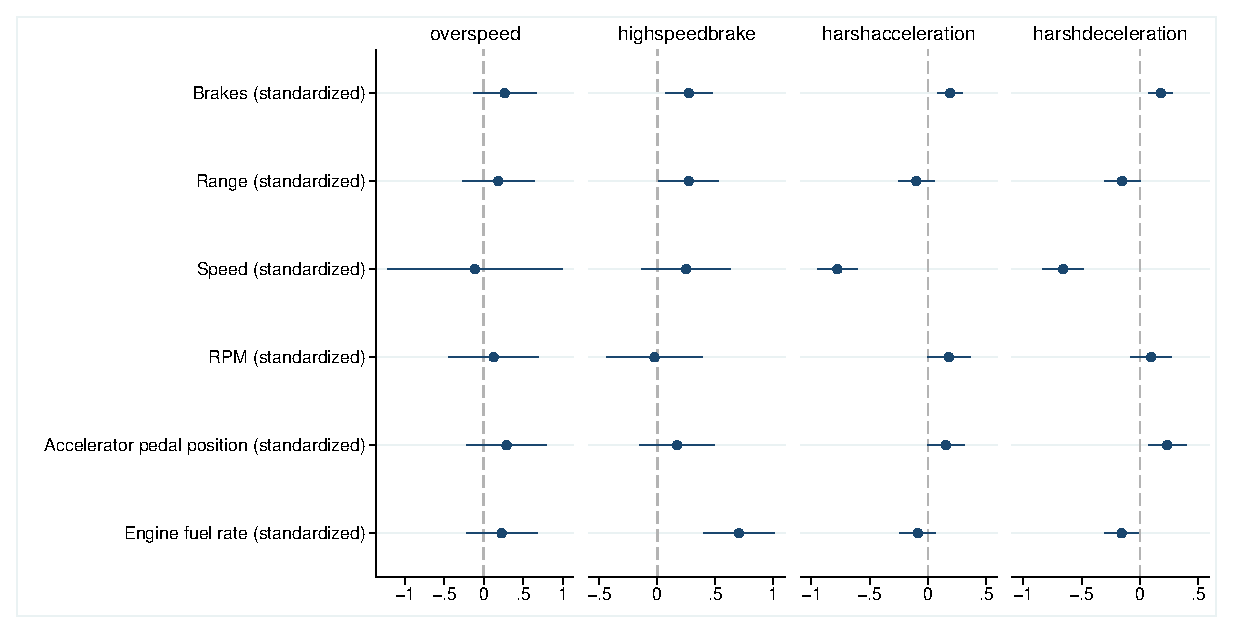
\includegraphics[width=1\columnwidth]{Figure/Coefplot1.eps}
    	\end{minipage}
		\label{coef_1}
    	}
	\\
	\subfigure[]{
		\begin{minipage}[t]{0.95\columnwidth}
		\centering
		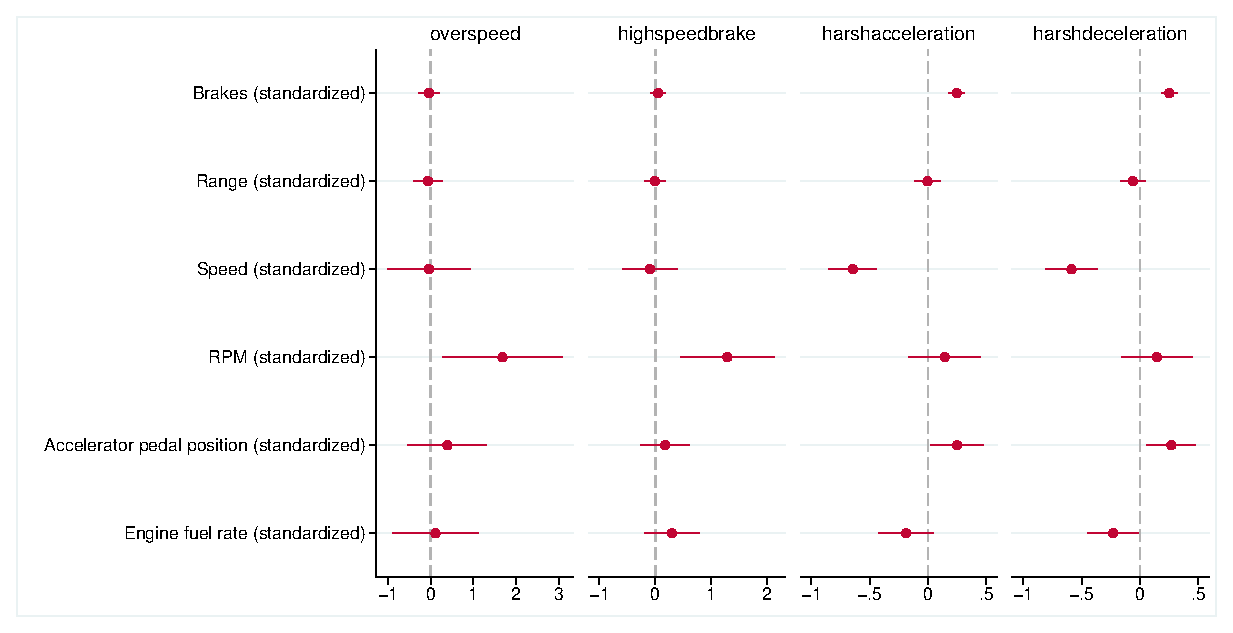
\includegraphics[width=1\columnwidth]{Figure/Coefplot2.eps}
		\end{minipage}
		\label{coef_2}
	}
	\caption{Partial coefficient estimation results of (a) Negative binomial regression; (b) Panel Negative binomial regression.}
	\label{coef}
\end{figure}
\begin{paracol}{2}
\linenumbers
\switchcolumn
%%%%%%%%%%%%%%%%%%%%%%%%%%%%%%%%%%%%%%%%%%
\subsection{Results of panel data set}
As shown in Table~\ref{comparison_xt}, the evaluation index(log-likelihood, AIC and BIC) of Negative binomial regression is lower than that of Poisson regression under each dependent variable. Therefore, Negative binomial regression is better than Poisson regression on panel data.
\end{paracol}
\begin{specialtable}[htbp]
\widetable
\caption{Model performances of Poisson and Negative binomial in the panel data set of drivers with six observations per driver.}
\label{comparison_xt}
\begin{tabular}{ccccccc}
\toprule
Variable                           & Model & N    & log-likelihood & df  & AIC      & BIC      \\
\midrule
\multirow{2}{*}{overspeed}         & XTPOS & 1092 & -1926.78       & 188 & 4229.559 & 5168.763 \\
                                   & XTNB  & 1092 & -957.497       & 189 & 2292.993 & 3237.193 \\

\multirow{2}{*}{highspeedbrake}    & XTPOS & 1092 & -2594.37       & 188 & 5564.733 & 6503.937 \\
                                   & XTNB  & 1092 & -1527.05       & 189 & 3432.105 & 4376.305 \\

\multirow{2}{*}{harshacceleration} & XTPOS & 1092 & -6117.44       & 188 & 12610.89 & 13550.09 \\
                                   & XTNB  & 1092 & -3526.09       & 189 & 7430.186 & 8374.386 \\

\multirow{2}{*}{harshdeceleration} & XTPOS & 1092 & -6042.02       & 188 & 12460.03 & 13399.24 \\
                                   & XTNB  & 1092 & -3547.66       & 189 & 7473.311 & 8417.51\\
\bottomrule
\end{tabular}
\end{specialtable}
\begin{paracol}{2}
\linenumbers
\switchcolumn
The panel Negative binomial regression was used to estimate the two-way fixed effect model considering both individual effect and time effect on four dependent variables. The influencing factors reflected by it (see Table~A\ref{panel-nb} and Figure~\ref{coef_2}) are not all the same as the results of summary data. What remains is that rapid acceleration and rapid deceleration are positively affected by the number of brakes (0.246 \& 0.253) and average accelerator pedal position (0.249 \& 0.270) but negatively affected by the average speed (-0.645 \& -0.586) and average engine fuel rate (-0.188 \& -0.229). However, RPM which is not significant in the summary data is significantly positive for over speed (1.683) and high speed braking (1.287). The brakes (0.0505) and engine fuel rate (0.295), which had a significant positive effect on the summary data, become insignificant.

The advantage of panel data over summary data is that fixed effects can be estimated and thus individual effects and time effects can be interpreted. The time effect are significant in most cases for high speed braking, rapid acceleration and rapid deceleration, which indicates that these three near-miss events are greatly influenced by time. The time effect of the over speed event is significant for only one day, suggesting that it is less influenced by time. Most importantly, the individual effects of the four near-miss events can be used to score each observation. It should be noted that the first individual has been omitted in the regression to avoid complete multicollinearity, and its coefficient value is expected to be zero used in the subsequent driving risk classification.
%%%%%%%%%%%%%%%%%%%%%%%%%%%%%%%%%%%%%%%%%%
\section{Discussions and Conclusions}

The results obtained by panel regression were more reliable than those obtained by pooled regression. Table~\ref{summary-nb}, Table~A\ref{panel-nb} and Figure~\ref{coef} show that some coefficient are not significant in the pooled Negative binomial regression become significant in the panel Negative binomial regression, while some significant parameters in the pooled Negative binomial regression become not significant in the panel Negative binomial regression. It means that the dependent variables are affected by individual effects and time effects. Most of the individual and time coefficients in the panel Negative binomial regression are significant, which indicates the effectiveness of the panel negative binomial regression.

Driving risks can be evaluated by the regression coefficients of Negative binomial models on panel data. The value of the individual coefficients within a regression indicates the individual's deviance from the level of the expected number of  such a near-miss event, given the information on all the other explanatory variables. In other words, the individual effect coefficient can be understood as the effect utility of each vehicle on the occurrence of the corresponding near-miss event. Geometrically, the effect coefficient of each individual is a change in the intercept.

Four near-miss events have been used as dependent variables to obtain four sets of regression coefficients. Given the influencing factors and generating mechanisms of different near-miss events are different, it is not recommended to combine the four groups of regression coefficients into one group. However, sharp acceleration and sharp deceleration show very similar characteristics in terms of data description before regression (Table~\ref{summary},\ref{summary-nb}), results after regression (Figure~\ref{coef} and Table~A\ref{panel-nb}) and distribution of driving risk score (Figure~\ref{score}), so it is feasible to combine them into a single near-miss event for further research.

In order to transform individual effect estimates of near-miss models into a driving risk grading, several steps need to be done. Firstly, winsorization avoids the influence of possibly spurious outliers (the double tail was winsorized with the threshold 0.01 in this study). Secondly, the regression coefficient can be compressed to the interval of [0,1] through normalization. Then, each group of coefficients is mapped into an interval of [0,5] (see Table~A\ref{score}), each observation then gets a driving risk level from 1 to 5, i.e. excellent, good, medium, bad and terrible (see Figure~\ref{rank}). To be clear, the values of exactly 0 and 5 are because the corresponding observations are the minimum and the maximum values in their group and are Min-Max scaled. In $overspeed$ and $highspeedbrake$ groups, two types of observations with high risk or low risk can be clearly seen. It indicates that these two near-miss events are more sensitive to driving behavior than $harshacceleration$ and $harshdeceleration$ and can be considered with higher priority and weight in subsequent studies. Note that the same observation (id125) has different risk levels for different near-miss events, which also explains why multiple near-miss events cannot be analyzed together. Ultimately, the premium will be charged individually according to the driving risk level of the insured one.

\end{paracol}
\begin{figure}[htbp]
\widefigure
\includegraphics[width=1\textwidth]{Figure/Rank.eps}
\caption{Driving risk rank of four near-miss events.}
\label{rank}
\end{figure}
\begin{paracol}{2}
\linenumbers
\switchcolumn

The number and type of dependent variables and independent variables selected in this study are limited by the size and quality of the original data. With the promotion and innovation of IoV and  of new energy vehicles, the amount and dimension of data will be greatly increased. Therefore, near-miss events as dependent variables could be increased or decreased flexibly according to needs. For example, it is recommended to include sharp turn as a near-miss event if possible, because sharp turn is highly studied and accident-proven patterns of high driving risk. For the same reason, more driving behavior indicators such as steering wheel angle speed, brake pedal position and so on could be used as independent variables in the regression model. In addition, traditional auto insurance factors such as driver information, vehicle information, road information, environment information and the health status of batteries (of new energy vehicles) should be considered to provide more optional independent variables for the model.

Econometrics and machine learning complement each other. The generalized linear model established in this study reveals the relationship between driving behavior factors and near-miss events, and gives a driving risk score for each observation. This model has strong explanatory power, but its generalization degree and robustness need to be further tested, especially when the data volume and data dimension are particularly large. The successful application of machine learning methods in many fields also shows that they are often effective in dealing with big data problems, but the biggest problem is that machine learning can not be explained well, which is exactly what the insurance field values. Therefore, it is a new research direction of telematics data application to find a balance between econometrics and machine learning, so as to have both good explanability, good generalization ability, quick response ability,  etc.\cite{gao2021boosting,so2021synthetic}.

In practical applications, near-miss events can be combined with claims and accidents to accurately evaluate driving risks. This study proves that near-miss events can be used as driving risk scores when there is no claims and accidents. However, when claims or accidents exist, the driving risk score obtained from claims or accidents can be used as the basis for premium calculation, while the driving risk rating obtained from near-miss events can be used to remind and warn drivers to reduce the corresponding dangerous driving habits.

In general, near-miss events can provide insurers with effective risk information in the absence of claims and accident data. Negative binomial regression is the most suitable modeling method for near-miss events as dependent variables in our real case study. This study provides a technical reference for the promotion and development of PHYD ratemaking schemes.
%%%%%%%%%%%%%%%%%%%%%%%%%%%%%%%%%%%%%%%%%%
\vspace{6pt}

%%%%%%%%%%%%%%%%%%%%%%%%%%%%%%%%%%%%%%%%%%
%% optional
%\supplementary{The following are available online at \linksupplementary{s1}, Figure S1: title, Table S1: title, Video S1: title.}

% Only for the journal Methods and Protocols:
% If you wish to submit a video article, please do so with any other supplementary material.
% \supplementary{The following are available at \linksupplementary{s1}, Figure S1: title, Table S1: title, Video S1: title. A supporting video article is available at doi: link.}

%%%%%%%%%%%%%%%%%%%%%%%%%%%%%%%%%%%%%%%%%%
\authorcontributions{Conceptualization, S.S. and M.G.; methodology, M.G.; software, S.S.; validation, J.B., M.G. and A.M.P.-M; formal analysis, S.S.; investigation, S.S.; resources, M.G.; data curation, J.B.; writing---original draft preparation, S.S.; writing---review and editing, S.S.; visualization, S.S.; supervision, J.B. and M.G.; project administration, J.B.; funding acquisition, J.B. and S.S.. All authors have read and agreed to the published version of the manuscript.}

\funding{This research was granted by the Fundamental Research Funds for the Central Universities 2019YJS091.}

\dataavailability{This study is based on the original telematics data from China Satellite Navigation and Communications Co., Ltd., which could not be made public due to confidentiality agreements.}

\acknowledgments{S.S. thanks the China Scholarship Council for providing visiting research funds in the second institution. M.G. thanks ICREA Academia. All the authors thank China Satellite Navigation and Communications Co., Ltd. for providing the original telematics data set.}

\conflictsofinterest{The authors declare no conflict of interest. The funders had no role in the design of the study; in the collection, analyses, or interpretation of data; in the writing of the manuscript, or in the decision to publish the results.}

%% Optional
% \sampleavailability{Samples of the compounds ... are available from the authors.}

%%%%%%%%%%%%%%%%%%%%%%%%%%%%%%%%%%%%%%%%%%
%% Only for journal Encyclopedia
%\entrylink{The Link to this entry published on the encyclopedia platform.}

%%%%%%%%%%%%%%%%%%%%%%%%%%%%%%%%%%%%%%%%%%
%% Optional
\abbreviations{The following abbreviations are used in this manuscript:\\

\noindent
\begin{tabular}{@{}ll}
UBI & usage-based insurance\\
IoV & Internet of vehicles\\
PAYD & pay as you drive\\
PHYD & pay how you drive\\
MHYD & manage how you drive\\
POS & Poisson\\
ZIP & Zero-inflated Poisson\\
NB & Negative binomial\\
ZINB & Zero-inflated Negative binomial\\
XTPOS & Panel Poisson\\
XTNB & Panel Negative binomial\\
AIC & Akaike information criterion\\
BIC & Bayesian information criterion\\
\end{tabular}}

%%%%%%%%%%%%%%%%%%%%%%%%%%%%%%%%%%%%%%%%%%
%% Optional
\appendixtitles{no} % Leave argument "no" if all appendix headings stay EMPTY (then no dot is printed after "Appendix A"). If the appendix sections contain a heading then change the argument to "yes".
\appendixstart
\appendix
\section{}
\end{paracol}
\begin{center}
\begin{longtable}{ccccccccc}
\caption{Panel Negative binomial regression results for four near-miss events.}
\label{panel-nb}\\
\toprule
\multicolumn{1}{c}{\multirow{2}{*}{Variable}} & \multicolumn{2}{c}{overspeed} & \multicolumn{2}{c}{highspeedbrake} & \multicolumn{2}{c}{harshacceleration} & \multicolumn{2}{c}{harshdeceleration} \\
\multicolumn{1}{c}{}                          & coefficient   & z-statistics  & coefficient     & z-statistics     & coefficient       & z-statistics      & coefficient       & z-statistics      \\
\midrule
constant                                         & -3.768***     & (-8.68)       & -4.356***       & (-17.39)         & -2.284***         & (-25.13)          & -2.269***         & (-20.81)          \\
brakes                                        & -0.0400       & (-0.31)       & 0.0505          & (0.73)           & 0.246***          & (6.93)            & 0.253***          & (7.23)            \\
range                                         & -0.0637       & (-0.36)       & -0.0108         & (-0.12)          & -0.00410          & (-0.07)           & -0.0595           & (-1.09)           \\
speed                                         & -0.0405       & (-0.08)       & -0.0965         & (-0.39)          & -0.645***         & (-6.09)           & -0.586***         & (-5.24)           \\
rpm                                           & 1.683*        & (2.34)        & 1.287**         & (3.00)           & 0.143             & (0.91)            & 0.145             & (0.93)            \\
acceleratorpedalposition                      & 0.391         & (0.83)        & 0.175           & (0.79)           & 0.249*            & (2.12)            & 0.270*            & (2.52)            \\
enginefuelrate                                & 0.113         & (0.22)        & 0.295           & (1.18)           & -0.188            & (-1.58)           & -0.229*           & (-2.04)           \\
2018-07-04                                    & 0.273         & (1.23)        & 0.216           & (1.91)           & -0.111*           & (-2.12)           & -0.216***         & (-4.33)           \\
2018-07-05                                    & -0.168        & (-0.73)       & -0.0572         & (-0.52)          & -0.206***         & (-4.34)           & -0.317***         & (-6.72)           \\
2018-07-06                                    & -0.00716      & (-0.03)       & -0.228*         & (-2.08)          & -0.257***         & (-4.84)           & -0.370***         & (-7.19)           \\
2018-07-07                                    & -0.477*       & (-2.11)       & -0.200          & (-1.68)          & -0.485***         & (-7.41)           & -0.600***         & (-9.27)           \\
2018-07-08                                    & 0.206         & (0.90)        & 0.117           & (0.95)           & -0.694***         & (-8.63)           & -0.784***         & (-9.58)           \\
id2                                           & -28.81***     & (-29.17)      & -2.001*         & (-2.25)          & 1.266***          & (5.24)            & 1.342***          & (4.80)            \\
id3                                           & -19.05***     & (-14.86)      & -18.13***       & (-16.37)         & 2.004*            & (2.31)            & 1.740***          & (4.75)            \\
id4                                           & -18.29***     & (-15.94)      & -17.91***       & (-20.04)         & 1.891***          & (8.66)            & 1.960***          & (8.58)            \\
id5                                           & -29.62***     & (-41.07)      & -4.956***       & (-7.51)          & -1.193***         & (-3.77)           & -1.072***         & (-3.39)           \\
id6                                           & -1.478*       & (-2.40)       & -0.554          & (-1.79)          & 1.067***          & (3.31)            & 0.935***          & (4.27)            \\
id7                                           & -3.236***     & (-4.11)       & -0.645          & (-1.58)          & 0.656**           & (3.15)            & 0.835**           & (3.05)            \\
id8                                           & -20.79***     & (-24.48)      & -2.368***       & (-4.01)          & -0.190            & (-0.61)           & 0.124             & (0.35)            \\
id9                                           & -1.156        & (-1.10)       & -0.0678         & (-0.11)          & -0.251            & (-0.79)           & -0.109            & (-0.28)           \\
id10                                          & -3.110***     & (-5.93)       & -1.527***       & (-4.20)          & -0.345*           & (-2.17)           & -0.256            & (-1.63)           \\
id11                                          & -2.026*       & (-2.42)       & -1.163***       & (-3.45)          & -0.162            & (-0.88)           & -0.272            & (-1.22)           \\
id12                                          & -1.342*       & (-2.51)       & -0.772*         & (-2.45)          & 0.0781            & (0.34)            & 0.0981            & (0.50)            \\
id13                                          & -2.344***     & (-5.13)       & -0.808*         & (-2.21)          & -0.138            & (-0.52)           & -0.129            & (-0.66)           \\
id14                                          & -3.178***     & (-5.87)       & 0.442           & (1.43)           & -0.629***         & (-3.66)           & -0.365*           & (-2.07)           \\
id15                                          & -1.254*       & (-2.31)       & 0.167           & (0.46)           & -0.0894           & (-0.34)           & 0.0270            & (0.10)            \\
id16                                          & -22.40***     & (-37.49)      & -21.63***       & (-41.20)         & 0.271             & (1.35)            & 0.439*            & (2.13)            \\
id17                                          & -21.77***     & (-25.73)      & -2.102***       & (-4.06)          & -0.200            & (-0.87)           & 0.0983            & (0.38)            \\
id18                                          & -20.99***     & (-19.61)      & -0.805          & (-1.48)          & -1.124***         & (-6.78)           & -1.267***         & (-5.69)           \\
id19                                          & -0.998        & (-1.58)       & 0.380           & (1.06)           & 0.587**           & (2.72)            & 0.586***          & (3.89)            \\
id20                                          & -23.99***     & (-38.51)      & -3.749**        & (-3.22)          & 0.292             & (1.19)            & 0.0926            & (0.40)            \\
id21                                          & -21.79***     & (-35.89)      & -2.577**        & (-2.75)          & 0.322             & (1.34)            & 0.458**           & (2.61)            \\
id22                                          & -2.642***     & (-3.94)       & -0.229          & (-0.63)          & 0.496**           & (3.00)            & 0.538**           & (2.89)            \\
id23                                          & -0.792        & (-1.10)       & 0.00108         & (0.00)           & -0.474            & (-1.61)           & -0.409            & (-1.71)           \\
id24                                          & -23.37***     & (-34.65)      & -22.27***       & (-40.12)         & -0.329            & (-1.36)           & -0.103            & (-0.32)           \\
id25                                          & -21.06***     & (-30.30)      & -20.67***       & (-32.16)         & -0.882***         & (-3.45)           & -0.731*           & (-2.56)           \\
id26                                          & -2.739***     & (-3.82)       & -1.000**        & (-2.61)          & -0.440            & (-1.77)           & -0.667***         & (-3.68)           \\
id27                                          & -23.10***     & (-41.71)      & -22.25***       & (-45.16)         & -0.0464           & (-0.15)           & 0.0656            & (0.22)            \\
id28                                          & -17.86***     & (-17.18)      & -17.85***       & (-18.78)         & 0.0432            & (0.13)            & 0.309             & (1.41)            \\
id29                                          & -1.136        & (-1.59)       & -0.872*         & (-2.33)          & 0.591***          & (3.74)            & 0.625***          & (4.09)            \\
id30                                          & -20.56***     & (-29.51)      & -19.84***       & (-31.89)         & -0.223            & (-0.53)           & -0.102            & (-0.25)           \\
id31                                          & -0.407        & (-0.91)       & -0.633*         & (-2.03)          & -1.148***         & (-3.69)           & -0.949**          & (-3.21)           \\
id32                                          & -3.255**      & (-3.24)       & -2.923*         & (-2.38)          & -0.110            & (-0.36)           & 0.143             & (0.49)            \\
id33                                          & -19.05***     & (-19.59)      & -19.50***       & (-21.06)         & -0.177            & (-0.37)           & -0.153            & (-0.32)           \\
id34                                          & -2.431**      & (-3.26)       & -1.547***       & (-3.51)          & -0.00573          & (-0.02)           & -0.0439           & (-0.14)           \\
id35                                          & -3.832***     & (-3.98)       & -1.041*         & (-2.18)          & -0.607***         & (-3.58)           & -0.552**          & (-3.14)           \\
id36                                          & -4.135***     & (-4.74)       & -2.412***       & (-4.36)          & -0.285            & (-1.37)           & -0.343            & (-1.82)           \\
id37                                          & -38.70***     & (-32.02)      & -1.232          & (-1.72)          & -0.480            & (-1.64)           & -0.218            & (-0.75)           \\
id38                                          & -20.26***     & (-29.14)      & -1.364*         & (-2.11)          & -1.484***         & (-5.08)           & -1.121***         & (-4.31)           \\
id39                                          & -38.61***     & (-41.67)      & 10.89***        & (14.67)          & 11.65***          & (21.85)           & 11.77***          & (21.58)           \\
id40                                          & -1.326        & (-1.57)       & -0.416          & (-0.81)          & -0.278            & (-1.10)           & 0.0791            & (0.30)            \\
id41                                          & -2.443**      & (-3.19)       & -1.020*         & (-2.02)          & 0.180             & (0.82)            & 0.155             & (0.61)            \\
id42                                          & -0.467        & (-0.57)       & 0.442           & (0.93)           & 0.607             & (1.63)            & 0.398             & (1.45)            \\
id43                                          & -2.164*       & (-2.45)       & 0.219           & (0.39)           & -0.0359           & (-0.13)           & 0.0900            & (0.35)            \\
id44                                          & -2.465***     & (-3.52)       & -0.156          & (-0.35)          & 0.336             & (1.33)            & 0.468             & (1.85)            \\
id45                                          & -2.110**      & (-3.26)       & -1.315**        & (-3.20)          & 0.105             & (0.64)            & 0.282             & (1.18)            \\
id46                                          & 0.132         & (0.14)        & -0.480          & (-1.01)          & -0.312**          & (-2.77)           & -0.235            & (-1.65)           \\
id47                                          & -2.957***     & (-5.23)       & -0.975          & (-1.32)          & -0.853***         & (-4.77)           & -0.656***         & (-4.01)           \\
id48                                          & 0.486         & (0.78)        & 1.381***        & (3.72)           & 0.829***          & (5.36)            & 0.787***          & (4.63)            \\
id49                                          & -25.28***     & (-34.70)      & -1.575**        & (-3.27)          & -0.568**          & (-2.60)           & -0.353            & (-1.67)           \\
id50                                          & -2.556***     & (-3.94)       & -1.907***       & (-3.87)          & -0.413*           & (-2.43)           & -0.331            & (-1.80)           \\
id51                                          & -20.62***     & (-20.07)      & -20.01***       & (-27.73)         & 1.123***          & (3.56)            & 1.140***          & (3.69)            \\
id52                                          & -21.73***     & (-16.76)      & -20.90***       & (-19.35)         & -0.354            & (-1.10)           & -0.952***         & (-3.75)           \\
id53                                          & -20.65***     & (-21.34)      & -20.00***       & (-31.74)         & -0.133            & (-0.72)           & 0.200             & (1.01)            \\
id54                                          & -4.881***     & (-5.39)       & -1.082**        & (-2.66)          & -0.686***         & (-3.36)           & -0.639**          & (-3.00)           \\
id55                                          & -4.290***     & (-4.44)       & -1.731***       & (-3.90)          & 0.472             & (1.80)            & 0.476             & (1.37)            \\
id56                                          & -2.462***     & (-3.72)       & -0.0866         & (-0.20)          & 0.119             & (0.40)            & 0.377             & (0.77)            \\
id57                                          & -21.96***     & (-22.99)      & -0.700          & (-1.51)          & 0.110             & (0.36)            & 0.719*            & (2.27)            \\
id58                                          & -1.877        & (-1.66)       & -0.692          & (-0.83)          & -0.344            & (-0.77)           & 0.0660            & (0.16)            \\
id59                                          & -38.77***     & (-43.77)      & -0.0709         & (-0.10)          & -0.726*           & (-2.11)           & -0.587            & (-1.68)           \\
id60                                          & -3.117**      & (-2.65)       & -3.815***       & (-4.00)          & -0.711*           & (-2.07)           & -0.565            & (-1.69)           \\
id61                                          & 0.821         & (0.83)        & 1.078           & (1.78)           & -1.288**          & (-2.87)           & -1.076*           & (-2.42)           \\
id62                                          & -0.465        & (-0.61)       & 0.546           & (1.46)           & -0.670            & (-1.58)           & -0.473            & (-1.15)           \\
id63                                          & -21.36***     & (-28.39)      & -20.68***       & (-33.84)         & 1.393***          & (10.47)           & 1.513***          & (10.22)           \\
id64                                          & -2.529        & (-1.39)       & -1.707          & (-1.18)          & 1.334***          & (7.83)            & 1.339***          & (6.13)            \\
id65                                          & -21.50***     & (-34.71)      & -20.76***       & (-42.35)         & -1.923***         & (-5.19)           & -1.288***         & (-5.26)           \\
id66                                          & -1.389        & (-1.49)       & -1.510***       & (-3.74)          & 0.504**           & (2.64)            & 0.971***          & (5.69)            \\
id67                                          & -25.65***     & (-34.83)      & -3.400***       & (-3.49)          & -0.371*           & (-1.98)           & -0.304            & (-1.70)           \\
id68                                          & -19.09***     & (-27.85)      & -18.66***       & (-35.37)         & -1.286**          & (-2.97)           & -1.660***         & (-7.16)           \\
id69                                          & -24.40***     & (-27.41)      & -21.86***       & (-33.37)         & -0.589**          & (-2.94)           & -0.625*           & (-2.48)           \\
id70                                          & -21.29***     & (-22.38)      & -3.693***       & (-4.50)          & -1.489***         & (-3.60)           & -1.501***         & (-6.37)           \\
id71                                          & -31.22***     & (-36.99)      & -29.36***       & (-53.20)         & 0.587***          & (3.95)            & 1.212***          & (7.82)            \\
id72                                          & -5.534***     & (-5.68)       & -1.058          & (-1.96)          & -0.516            & (-1.41)           & -0.643            & (-1.84)           \\
id73                                          & -4.323***     & (-4.06)       & -2.863***       & (-5.25)          & -1.527***         & (-6.22)           & -1.523***         & (-5.97)           \\
id74                                          & -30.92***     & (-35.40)      & -29.09***       & (-51.97)         & 0.299             & (1.03)            & 0.765**           & (3.02)            \\
id75                                          & -2.868***     & (-3.45)       & -1.677***       & (-4.49)          & -0.267            & (-0.90)           & -0.0911           & (-0.31)           \\
id76                                          & -21.21***     & (-22.83)      & -21.18***       & (-31.54)         & -1.646***         & (-3.80)           & -1.903***         & (-4.47)           \\
id77                                          & -19.83***     & (-15.23)      & -19.23***       & (-21.15)         & 0.835**           & (2.84)            & 0.729**           & (2.71)            \\
id78                                          & -24.02***     & (-33.62)      & -3.260***       & (-3.47)          & -2.855***         & (-10.67)          & -2.759***         & (-8.49)           \\
id79                                          & -3.449**      & (-2.81)       & -0.618          & (-1.43)          & -0.232            & (-1.23)           & -0.110            & (-0.57)           \\
id80                                          & -21.71***     & (-15.28)      & -20.69***       & (-20.65)         & -0.0149           & (-0.05)           & 0.0509            & (0.16)            \\
id81                                          & -33.98***     & (-60.17)      & -1.132*         & (-2.44)          & -0.341*           & (-2.34)           & -0.336*           & (-2.41)           \\
id82                                          & -1.391        & (-1.64)       & -0.541          & (-0.76)          & -0.312            & (-1.38)           & -0.326            & (-1.55)           \\
id83                                          & -1.516**      & (-2.58)       & 0.157           & (0.53)           & -0.123            & (-0.64)           & -0.242            & (-1.37)           \\
id84                                          & -23.95***     & (-25.81)      & -1.866*         & (-2.04)          & -0.750**          & (-3.19)           & -0.855***         & (-4.50)           \\
id85                                          & -22.55***     & (-23.68)      & -3.844***       & (-4.49)          & -1.430***         & (-5.83)           & -1.318***         & (-5.43)           \\
id86                                          & -29.06***     & (-33.35)      & -2.036***       & (-3.87)          & -1.272***         & (-3.40)           & -1.111**          & (-2.99)           \\
id87                                          & -1.851*       & (-2.47)       & 1.034**         & (2.59)           & 0.196             & (1.03)            & 0.425*            & (2.03)            \\
id88                                          & -20.13***     & (-31.73)      & -19.83***       & (-38.92)         & -0.208            & (-1.54)           & -0.165            & (-1.04)           \\
id89                                          & -25.42***     & (-13.08)      & -23.44***       & (-19.03)         & 1.100*            & (2.18)            & 1.135*            & (2.49)            \\
id90                                          & -4.008***     & (-4.24)       & -0.841          & (-1.18)          & -0.972***         & (-4.48)           & -0.982**          & (-3.17)           \\
id91                                          & -19.51***     & (-26.36)      & -19.33***       & (-31.18)         & 0.676***          & (5.52)            & 0.818***          & (4.54)            \\
id92                                          & -26.04***     & (-14.88)      & -24.17***       & (-22.56)         & 0.848*            & (2.54)            & 0.663*            & (2.00)            \\
id93                                          & -23.79***     & (-23.97)      & -22.53***       & (-27.69)         & -0.290            & (-1.41)           & -0.300            & (-1.26)           \\
id94                                          & -2.684***     & (-3.53)       & -1.034**        & (-3.05)          & -0.157            & (-0.99)           & 0.0139            & (0.06)            \\
id95                                          & -24.75***     & (-12.35)      & -22.86***       & (-19.16)         & -0.503            & (-0.78)           & -0.670            & (-1.26)           \\
id96                                          & -22.66***     & (-28.80)      & -21.77***       & (-35.98)         & 1.374***          & (7.81)            & 1.343***          & (6.60)            \\
id97                                          & -20.83***     & (-29.33)      & -20.42***       & (-32.43)         & -0.464*           & (-2.30)           & -0.282            & (-1.24)           \\
id98                                          & -18.59***     & (-24.60)      & -18.56***       & (-27.54)         & -1.405***         & (-4.98)           & -0.887*           & (-2.38)           \\
id99                                          & -18.19***     & (-27.16)      & -18.21***       & (-34.28)         & -1.774***         & (-5.28)           & -1.369***         & (-4.34)           \\
id100                                         & -4.226**      & (-3.13)       & -21.52***       & (-26.23)         & 0.802*            & (2.30)            & 0.824*            & (2.37)            \\
id101                                         & -22.60***     & (-13.70)      & -21.29***       & (-22.32)         & 0.955*            & (2.21)            & 0.814             & (1.96)            \\
id102                                         & -24.81***     & (-34.96)      & -23.71***       & (-42.27)         & 0.0308            & (0.14)            & -0.0294           & (-0.12)           \\
id103                                         & -17.82***     & (-22.56)      & -17.67***       & (-27.25)         & 0.542*            & (2.27)            & 0.606***          & (3.70)            \\
id104                                         & -20.05***     & (-32.16)      & -19.72***       & (-37.06)         & 0.131             & (0.73)            & 0.262*            & (1.98)            \\
id105                                         & -3.426***     & (-4.29)       & -0.430          & (-0.94)          & -0.464            & (-0.90)           & -0.925*           & (-2.01)           \\
id106                                         & -24.96***     & (-26.36)      & -23.73***       & (-35.39)         & 0.317             & (1.84)            & 0.252             & (1.33)            \\
id107                                         & -21.01***     & (-29.69)      & -20.53***       & (-36.62)         & 0.0144            & (0.09)            & 0.147             & (0.63)            \\
id108                                         & -23.28***     & (-27.56)      & -2.647***       & (-5.35)          & -0.532*           & (-2.40)           & -0.635***         & (-3.35)           \\
id109                                         & -20.89***     & (-19.32)      & -20.46***       & (-21.38)         & -0.347**          & (-2.97)           & -0.782***         & (-5.90)           \\
id110                                         & -20.70***     & (-17.96)      & -20.72***       & (-20.15)         & -1.801***         & (-5.72)           & -1.044***         & (-5.99)           \\
id111                                         & -3.405***     & (-4.19)       & -1.278***       & (-3.61)          & 0.173             & (1.27)            & 0.198             & (1.40)            \\
id112                                         & -19.65***     & (-24.23)      & -19.29***       & (-25.89)         & -1.453***         & (-8.75)           & -0.831***         & (-7.19)           \\
id113                                         & -29.63***     & (-42.75)      & -2.998***       & (-3.76)          & -1.703***         & (-6.85)           & -1.296***         & (-6.74)           \\
id114                                         & -23.43***     & (-20.14)      & -22.26***       & (-23.54)         & 0.637**           & (2.80)            & 0.537**           & (3.22)            \\
id115                                         & -22.18***     & (-29.89)      & -21.49***       & (-33.89)         & -0.0179           & (-0.14)           & -0.109            & (-0.69)           \\
id116                                         & -21.78***     & (-24.48)      & -3.753***       & (-7.41)          & -1.349***         & (-4.54)           & -1.135**          & (-2.79)           \\
id117                                         & -20.71***     & (-26.29)      & -20.08***       & (-32.28)         & -0.156            & (-1.35)           & -0.273*           & (-2.17)           \\
id118                                         & -18.97***     & (-27.81)      & -0.705          & (-0.91)          & 0.116             & (0.88)            & 0.00337           & (0.02)            \\
id119                                         & -20.31***     & (-30.19)      & -19.89***       & (-36.33)         & -0.145            & (-0.79)           & -0.143            & (-0.92)           \\
id120                                         & -27.27***     & (-33.83)      & -25.62***       & (-41.44)         & -0.0170           & (-0.06)           & 0.133             & (0.42)            \\
id121                                         & -28.62***     & (-36.09)      & -0.687          & (-1.76)          & 0.239             & (1.20)            & 0.387*            & (2.01)            \\
id122                                         & -21.69***     & (-15.37)      & -2.515*         & (-2.40)          & 0.623*            & (2.36)            & 0.653*            & (2.48)            \\
id123                                         & -23.18***     & (-12.54)      & -3.892***       & (-4.57)          & 0.698             & (1.51)            & 0.886*            & (2.13)            \\
id124                                         & -4.268*       & (-2.34)       & -2.612*         & (-2.50)          & 0.698**           & (2.66)            & 0.361             & (1.22)            \\
id125                                         & -3.828*       & (-2.35)       & -22.52***       & (-19.24)         & 0.296             & (0.67)            & 0.619             & (1.69)            \\
id126                                         & -2.023        & (-1.24)       & -2.183*         & (-2.54)          & 0.576             & (1.84)            & 0.539             & (1.73)            \\
id127                                         & -22.03***     & (-12.96)      & -20.58***       & (-19.98)         & 1.158***          & (4.23)            & 1.010***          & (3.82)            \\
id128                                         & -20.90***     & (-14.97)      & -20.01***       & (-22.10)         & 0.762**           & (2.84)            & 0.618*            & (2.18)            \\
id129                                         & -1.540*       & (-2.37)       & 0.776*          & (2.07)           & 0.0280            & (0.17)            & 0.165             & (0.76)            \\
id130                                         & -24.70***     & (-30.90)      & -23.31***       & (-35.06)         & -1.578***         & (-5.17)           & -1.635***         & (-4.61)           \\
id131                                         & -1.659*       & (-2.10)       & -0.403          & (-1.01)          & -0.980***         & (-3.71)           & -0.794***         & (-4.13)           \\
id132                                         & -19.37***     & (-26.07)      & -18.83***       & (-32.28)         & -0.863***         & (-3.40)           & -0.435            & (-1.85)           \\
id133                                         & -26.03***     & (-21.40)      & -2.904***       & (-8.09)          & -0.622***         & (-4.18)           & -0.691***         & (-4.38)           \\
id134                                         & -31.36***     & (-34.83)      & -2.618***       & (-5.23)          & 0.488*            & (2.40)            & 1.176***          & (6.93)            \\
id135                                         & -23.37***     & (-24.64)      & -22.02***       & (-35.69)         & 0.930***          & (4.58)            & 1.350***          & (7.18)            \\
id136                                         & 3.358***      & (3.79)        & 4.212***        & (6.07)           & 2.661***          & (8.38)            & 2.709***          & (11.14)           \\
id137                                         & -23.49***     & (-24.93)      & -2.508**        & (-2.65)          & 0.0440            & (0.26)            & 0.804***          & (4.16)            \\
id138                                         & -19.02***     & (-29.14)      & -18.74***       & (-37.30)         & -0.827***         & (-3.86)           & -0.890***         & (-3.54)           \\
id139                                         & -4.105***     & (-4.05)       & -1.187*         & (-2.54)          & -0.922**          & (-3.06)           & -0.677            & (-1.61)           \\
id140                                         & -2.970**      & (-3.06)       & -0.615          & (-1.10)          & -1.276***         & (-3.79)           & -1.035***         & (-3.61)           \\
id141                                         & -24.65***     & (-33.01)      & -23.40***       & (-44.51)         & -1.071***         & (-4.15)           & -1.100***         & (-4.52)           \\
id142                                         & -37.04***     & (-41.13)      & -0.873          & (-1.69)          & 0.0500            & (0.22)            & 0.175             & (0.76)            \\
id143                                         & -37.41***     & (-40.91)      & -0.397          & (-0.82)          & -0.368            & (-1.15)           & -0.157            & (-0.52)           \\
id144                                         & -0.585        & (-0.65)       & 0.551           & (1.04)           & 0.0261            & (0.09)            & 0.167             & (0.58)            \\
id145                                         & -2.485*       & (-2.36)       & -1.273*         & (-2.44)          & -0.750            & (-1.56)           & -0.631            & (-1.32)           \\
id146                                         & -22.93***     & (-26.06)      & -1.250**        & (-2.87)          & -1.130**          & (-2.83)           & -0.758*           & (-1.97)           \\
id147                                         & -2.851***     & (-3.75)       & -0.0796         & (-0.17)          & -1.021**          & (-2.90)           & -0.896**          & (-2.59)           \\
id148                                         & -3.737***     & (-4.05)       & 1.617***        & (3.83)           & -0.0483           & (-0.14)           & -0.0520           & (-0.16)           \\
id149                                         & -3.202***     & (-3.53)       & -1.184*         & (-2.01)          & -0.554**          & (-2.59)           & -0.343            & (-1.54)           \\
id150                                         & -3.616**      & (-3.24)       & -0.905*         & (-2.24)          & -1.167***         & (-4.30)           & -0.905***         & (-3.46)           \\
id151                                         & -0.362        & (-0.51)       & -1.167*         & (-2.07)          & -1.654***         & (-5.15)           & -1.677***         & (-4.32)           \\
id152                                         & -32.89***     & (-33.69)      & -3.751***       & (-6.31)          & -1.421***         & (-3.68)           & -1.382***         & (-4.40)           \\
id153                                         & -1.598*       & (-2.14)       & -0.169          & (-0.46)          & -2.936***         & (-5.34)           & -3.067***         & (-5.01)           \\
id154                                         & -21.84***     & (-20.17)      & -2.716***       & (-3.85)          & -1.703***         & (-4.38)           & -1.483***         & (-4.26)           \\
id155                                         & -4.238***     & (-3.67)       & -2.441*         & (-2.46)          & -0.759**          & (-3.12)           & -0.814**          & (-2.63)           \\
id156                                         & -43.11***     & (-52.10)      & -1.456**        & (-3.27)          & -0.590**          & (-2.64)           & -0.429*           & (-2.03)           \\
id157                                         & -1.868*       & (-2.19)       & 0.337           & (0.62)           & -0.753**          & (-2.82)           & -0.502*           & (-2.35)           \\
id158                                         & -19.28***     & (-28.14)      & -18.96***       & (-35.46)         & 0.678***          & (4.39)            & 0.744***          & (3.87)            \\
id159                                         & -19.26***     & (-28.40)      & -19.02***       & (-33.84)         & 0.827***          & (4.09)            & 0.715**           & (3.07)            \\
id160                                         & -3.790***     & (-4.60)       & 0.550           & (1.25)           & 0.148             & (0.72)            & 0.337             & (1.90)            \\
id161                                         & -22.11***     & (-30.73)      & -21.31***       & (-34.53)         & 0.608***          & (4.58)            & 0.494***          & (3.29)            \\
id162                                         & -20.15***     & (-18.45)      & -19.53***       & (-23.73)         & 0.431             & (1.86)            & 0.176             & (0.52)            \\
id163                                         & -22.31***     & (-22.00)      & -21.43***       & (-29.98)         & 1.844***          & (9.58)            & 1.656***          & (8.12)            \\
id164                                         & -2.923**      & (-2.69)       & -2.557***       & (-3.68)          & -0.245            & (-1.66)           & -0.301            & (-1.85)           \\
id165                                         & -20.82***     & (-28.93)      & -20.41***       & (-32.12)         & 1.341***          & (11.50)           & 1.447***          & (10.42)           \\
id166                                         & -25.44***     & (-20.51)      & -2.439***       & (-4.42)          & -0.158            & (-0.49)           & -0.0534           & (-0.15)           \\
id167                                         & -2.696*       & (-2.28)       & -4.124***       & (-4.21)          & 1.119***          & (3.43)            & 1.089***          & (3.53)            \\
id168                                         & -5.731***     & (-6.49)       & -1.940***       & (-3.42)          & 0.0447            & (0.23)            & 0.0115            & (0.06)            \\
id169                                         & -26.04***     & (-24.96)      & -24.71***       & (-35.44)         & 0.473*            & (2.06)            & 0.422             & (1.82)            \\
id170                                         & -15.15***     & (-15.82)      & -15.11***       & (-19.48)         & -17.48***         & (-24.79)          & -0.684            & (-0.99)           \\
id171                                         & -3.650***     & (-3.49)       & -1.497**        & (-2.86)          & -0.344            & (-1.62)           & -0.313            & (-1.47)           \\
id172                                         & -3.659***     & (-3.93)       & -1.951***       & (-4.53)          & -0.427            & (-1.84)           & -0.367            & (-1.34)           \\
id173                                         & -3.036**      & (-2.98)       & -3.500***       & (-4.94)          & -0.874***         & (-3.64)           & -0.888***         & (-3.41)           \\
id174                                         & 1.453         & (1.39)        & 0.361           & (0.38)           & -1.484***         & (-6.68)           & -1.288***         & (-4.64)           \\
id175                                         & -0.688        & (-0.99)       & 1.615***        & (3.66)           & 0.114             & (0.57)            & 0.333             & (1.64)            \\
id176                                         & -1.666        & (-1.82)       & -0.313          & (-0.81)          & 0.530             & (0.98)            & -0.0614           & (-0.13)           \\
id177                                         & -2.576**      & (-3.13)       & -1.675***       & (-3.66)          & -0.245            & (-1.10)           & 0.187             & (0.75)            \\
id178                                         & -0.823        & (-0.51)       & 0.510           & (1.04)           & 0.213             & (1.00)            & 0.0436            & (0.18)            \\
id179                                         & -19.54***     & (-27.56)      & -1.071          & (-1.13)          & -1.386***         & (-4.24)           & -1.021            & (-1.91)           \\
id180                                         & -4.457***     & (-3.85)       & -2.934***       & (-3.90)          & -0.402*           & (-2.17)           & -0.277            & (-1.44)           \\
id181                                         & -1.850*       & (-2.18)       & -0.909*         & (-2.21)          & -0.573            & (-1.78)           & -0.354            & (-1.41)           \\
id182                                         & -4.754**      & (-3.03)       & -2.082**        & (-2.75)          & 0.387             & (1.35)            & 0.409             & (1.60)            \\
log-likelihood     & \multicolumn{2}{c}{-952.2391} & \multicolumn{2}{c}{-1519.954}      & \multicolumn{2}{c}{-3479.969}         & \multicolumn{2}{c}{-3488.38}          \\
AIC                      & \multicolumn{2}{c}{2292.478}  & \multicolumn{2}{c}{3427.908}       & \multicolumn{2}{c}{7347.937}          & \multicolumn{2}{c}{7364.76}           \\
BIC                      & \multicolumn{2}{c}{3261.657}  & \multicolumn{2}{c}{4397.086}       & \multicolumn{2}{c}{8317.116}          & \multicolumn{2}{c}{8333.939}          \\
Observations             & \multicolumn{2}{c}{1092}     & \multicolumn{2}{c}{1092}          & \multicolumn{2}{c}{1092}             & \multicolumn{2}{c}{1092}\\
\bottomrule
\footnotesize{$^a$ *** p<0.01, ** p<0.05, * p<0.1}
\end{longtable}
\end{center}

\begin{center}
\begin{longtable}{ccccc}
\caption{Driving risk scores for four near-miss events after winsorizing and Min-Max scaling on regression coefficients.}
\label{score}\\
\toprule
Variable & overspeed & highspeedbrake & harshacceleration & harshdeceleration \\
\midrule
id1       & 4.824741  & 4.344986       & 2.622834          & 2.52286           \\
id2       & 1.242371  & 4.033808       & 3.753797          & 3.75              \\
id3       & 2.476298  & 1.628204       & 4.413078          & 4.113936          \\
id4       & 2.578824  & 1.749502       & 4.312131          & 4.315106          \\
id5       & 1.133814  & 3.574272       & 1.557084          & 1.542612          \\
id6       & 4.646467  & 4.258833       & 3.576023          & 3.377835          \\
id7       & 4.434299  & 4.244682       & 3.208862          & 3.286394          \\
id8       & 2.244711  & 3.976736       & 2.4531            & 2.636247          \\
id9       & 4.685306  & 4.334427       & 2.398606          & 2.423189          \\
id10      & 4.449618  & 4.107521       & 2.314633          & 2.288771          \\
id11      & 4.580368  & 4.164127       & 2.478113          & 2.27414           \\
id12      & 4.662871  & 4.224932       & 2.692603          & 2.612564          \\
id13      & 4.542011  & 4.219333       & 2.499553          & 2.404901          \\
id14      & 4.441416  & 4.413722       & 2.060925          & 2.1891            \\
id15      & 4.673486  & 4.370957       & 2.542969          & 2.547549          \\
id16      & 2.050515  & 1.186551       & 2.864928          & 2.924287          \\
id17      & 2.12168   & 4.018102       & 2.444167          & 2.612747          \\
id18      & 2.218175  & 4.2198         & 1.618724          & 1.364301          \\
id19      & 4.704364  & 4.404081       & 3.147222          & 3.058705          \\
id20      & 1.835814  & 3.761974       & 2.883688          & 2.607535          \\
id21      & 2.124092  & 3.944234       & 2.910488          & 2.941661          \\
id22      & 4.506067  & 4.309374       & 3.065928          & 3.014813          \\
id23      & 4.729211  & 4.345159       & 2.199393          & 2.148866          \\
id24      & 1.923866  & 1.063697       & 2.328926          & 2.428676          \\
id25      & 2.207319  & 1.317181       & 1.834912          & 1.854426          \\
id26      & 4.494367  & 4.189475       & 2.229766          & 1.912948          \\
id27      & 1.957639  & 1.080804       & 2.581383          & 2.582846          \\
id28      & 2.621041  & 1.695073       & 2.661426          & 2.805413          \\
id29      & 4.687598  & 4.20938        & 3.150795          & 3.094367          \\
id30      & 2.274866  & 1.419818       & 2.42362           & 2.42959           \\
id31      & 4.77565   & 4.246703       & 1.597284          & 1.655084          \\
id32      & 4.432128  & 3.890427       & 2.524567          & 2.653621          \\
id33      & 2.476298  & 1.503794       & 2.464713          & 2.382955          \\
id34      & 4.531518  & 4.10441        & 2.617715          & 2.482718          \\
id35      & 4.362531  & 4.183099       & 2.080579          & 2.018105          \\
id36      & 4.325984  & 3.970049       & 2.368233          & 2.209217          \\
id37      & 0.021711  & 4.153396       & 2.194033          & 2.323519          \\
id38      & 2.317082  & 4.132869       & 1.297123          & 1.497805          \\
id39      & 0.024124  & 5              & 5                 & 5                 \\
id40      & 4.664922  & 4.280294       & 2.374486          & 2.59519           \\
id41      & 4.53007   & 4.186365       & 2.783634          & 2.664594          \\
id42      & 4.768412  & 4.413722       & 3.165088          & 2.886796          \\
id43      & 4.563723  & 4.379043       & 2.590763          & 2.605157          \\
id44      & 4.527417  & 4.320727       & 2.922994          & 2.950805          \\
id45      & 4.570236  & 4.140489       & 2.716634          & 2.780724          \\
id46      & 4.840663  & 4.270341       & 2.344113          & 2.307974          \\
id47      & 4.468072  & 4.193363       & 1.860818          & 1.923007          \\
id48      & 4.883362  & 4.559747       & 3.363409          & 3.242502          \\
id49      & 1.672979  & 4.100056       & 2.115419          & 2.200073          \\
id50      & 4.51644   & 4.048426       & 2.253886          & 2.22019           \\
id51      & 2.268835  & 1.384051       & 3.62605           & 3.565289          \\
id52      & 2.192845  & 1.124347       & 2.306593          & 1.652341          \\
id53      & 2.260391  & 1.348283       & 2.50402           & 2.705743          \\
id54      & 4.236002  & 4.176723       & 2.010005          & 1.938552          \\
id55      & 4.307288  & 4.075796       & 3.044488          & 2.95812           \\
id56      & 4.527778  & 4.331519       & 2.729141          & 2.867593          \\
id57      & 2.18802   & 4.236128       & 2.721101          & 3.180322          \\
id58      & 4.59834   & 4.237372       & 2.315526          & 2.583211          \\
id59      & 0         & 4.333961       & 1.974272          & 1.986101          \\
id60      & 4.448773  & 3.752022       & 1.987672          & 2.006218          \\
id61      & 4.923769  & 4.512628       & 1.472217          & 1.538954          \\
id62      & 4.768654  & 4.429895       & 2.024299          & 2.090344          \\
id63      & 2.165103  & 1.309405       & 3.86725           & 3.906364          \\
id64      & 4.519697  & 4.079528       & 3.814544          & 3.747257          \\
id65      & 2.171134  & 1.334287       & 0.904949          & 1.345099          \\
id66      & 4.657202  & 4.110164       & 3.073075          & 3.410753          \\
id67      & 1.641618  & 3.816248       & 2.291406          & 2.244879          \\
id68      & 2.459412  & 1.607987       & 1.474004          & 1.004938          \\
id69      & 1.78636   & 1.116571       & 2.096659          & 1.951353          \\
id70      & 2.194051  & 3.770683       & 1.292657          & 1.150329          \\
id71      & 0.937206  & 0              & 3.147222          & 3.631127          \\
id72      & 4.157238  & 4.180455       & 2.161872          & 1.934894          \\
id73      & 4.303307  & 3.899757       & 1.25871           & 1.130212          \\
id74      & 0.979422  & 0              & 2.889941          & 3.222385          \\
id75      & 4.478807  & 4.084194       & 2.384313          & 2.439557          \\
id76      & 2.198876  & 0.898855       & 1.152403          & 0.782736          \\
id77      & 2.366536  & 1.433814       & 3.368769          & 3.189466          \\
id78      & 1.845464  & 3.838019       & 0.07236           & 0                 \\
id79      & 4.408728  & 4.24888        & 2.41558           & 2.422275          \\
id80      & 2.130123  & 1.197437       & 2.609523          & 2.569404          \\
id81      & 0.595856  & 4.168947       & 2.318206          & 2.215618          \\
id82      & 4.656961  & 4.260855       & 2.344113          & 2.224762          \\
id83      & 4.641884  & 4.369402       & 2.512953          & 2.301573          \\
id84      & 1.823752  & 4.054802       & 1.952832          & 1.741039          \\
id85      & 2.061371  & 3.747356       & 1.345364          & 1.317666          \\
id86      & 1.21101   & 4.028365       & 1.486511          & 1.50695           \\
id87      & 4.601476  & 4.505785       & 2.797927          & 2.911485          \\
id88      & 2.341206  & 1.475802       & 2.43702           & 2.371982          \\
id89      & 1.641618  & 0.869308       & 3.605503          & 3.560717          \\
id90      & 4.341302  & 4.214201       & 1.754511          & 1.624909          \\
id91      & 2.40634   & 1.387161       & 3.226729          & 3.270849          \\
id92      & 1.571659  & 0.774446       & 3.380382          & 3.129115          \\
id93      & 1.873206  & 1.03415        & 2.363766          & 2.248537          \\
id94      & 4.501001  & 4.184188       & 2.48258           & 2.535571          \\
id95      & 1.736907  & 0.925292       & 2.173486          & 1.910205          \\
id96      & 1.999855  & 1.163225       & 3.850277          & 3.750914          \\
id97      & 2.23868   & 1.320291       & 2.208326          & 2.264996          \\
id98      & 2.526958  & 1.600211       & 1.367697          & 1.711778          \\
id99      & 2.583649  & 1.687298       & 1.038056          & 1.271031          \\
id100     & 4.315007  & 1.200547       & 3.339289          & 3.276335          \\
id101     & 2.014329  & 1.197437       & 3.475969          & 3.267191          \\
id102     & 1.72967   & 0.847537       & 2.650348          & 2.495977          \\
id103     & 2.619835  & 1.71218        & 3.107022          & 3.076993          \\
id104     & 2.34      & 1.460251       & 2.739861          & 2.762436          \\
id105     & 4.411502  & 4.278116       & 2.208326          & 1.67703           \\
id106     & 1.711577  & 0.852202       & 2.906021          & 2.753292          \\
id107     & 2.215762  & 1.324956       & 2.635698          & 2.657279          \\
id108     & 1.917835  & 3.933348       & 2.147579          & 1.942209          \\
id109     & 2.236268  & 1.290744       & 2.312846          & 1.807791          \\
id110     & 2.288134  & 1.175666       & 1.013936          & 1.568215          \\
id111     & 4.414035  & 4.146398       & 2.777381          & 2.703914          \\
id112     & 2.390659  & 1.522456       & 1.324817          & 1.762985          \\
id113     & 1.147082  & 3.878919       & 1.101483          & 1.337783          \\
id114     & 1.90336   & 1.068363       & 3.191889          & 3.013899          \\
id115     & 2.062577  & 1.197437       & 2.606843          & 2.423189          \\
id116     & 2.119268  & 3.761352       & 1.417724          & 1.485004          \\
id117     & 2.253154  & 1.382496       & 2.483473          & 2.273226          \\
id118     & 2.469061  & 4.235351       & 2.726461          & 2.525942          \\
id119     & 2.30502   & 1.421373       & 2.4933            & 2.392099          \\
id120     & 1.435361  & 0.55051        & 2.607647          & 2.644477          \\
id121     & 1.255639  & 4.23815        & 2.836341          & 2.876737          \\
id122     & 2.133742  & 3.953875       & 3.179382          & 3.119971          \\
id123     & 1.987793  & 3.739736       & 3.246382          & 3.333029          \\
id124     & 4.309941  & 3.938791       & 3.246382          & 2.852963          \\
id125     & 4.363014  & 1.066808       & 2.887261          & 3.088881          \\
id126     & 4.58073   & 4.005505       & 3.137395          & 3.015728          \\
id127     & 2.083082  & 1.265862       & 3.657316          & 3.446416          \\
id128     & 2.225412  & 1.262752       & 3.303555          & 3.087966          \\
id129     & 4.638989  & 4.465819       & 2.647847          & 2.673738          \\
id130     & 1.741732  & 0.892635       & 1.21315           & 1.027798          \\
id131     & 4.624635  & 4.282315       & 1.747365          & 1.796818          \\
id132     & 2.42202   & 1.567554       & 1.851885          & 2.125091          \\
id133     & 1.568041  & 3.893381       & 2.067179          & 1.891002          \\
id134     & 0.916701  & 3.937858       & 3.058781          & 3.598208          \\
id135     & 1.906979  & 1.087024       & 3.453636          & 3.757315          \\
id136     & 5         & 5              & 5                 & 5                 \\
id137     & 1.893711  & 3.954964       & 2.66214           & 3.258047          \\
id138     & 2.485948  & 1.635979       & 1.884045          & 1.709034          \\
id139     & 4.329602  & 4.160394       & 1.799178          & 1.903804          \\
id140     & 4.466504  & 4.249347       & 1.482937          & 1.576445          \\
id141     & 1.759824  & 0.892635       & 1.666071          & 1.517008          \\
id142     & 0.219526  & 4.209225       & 2.6675            & 2.682882          \\
id143     & 0.171278  & 4.283248       & 2.294086          & 2.379298          \\
id144     & 4.754179  & 4.430673       & 2.64615           & 2.675567          \\
id145     & 4.525004  & 4.14702        & 1.952832          & 1.945867          \\
id146     & 1.947989  & 4.150597       & 1.613364          & 1.829737          \\
id147     & 4.480858  & 4.332608       & 1.710738          & 1.703548          \\
id148     & 4.37399   & 4.596448       & 2.579686          & 2.475311          \\
id149     & 4.438521  & 4.160861       & 2.127926          & 2.209217          \\
id150     & 4.388585  & 4.204249       & 1.580311          & 1.695318          \\
id151     & 4.781077  & 4.163505       & 1.145256          & 0.989393          \\
id152     & 0.724917  & 3.761663       & 1.353404          & 1.259144          \\
id153     & 4.631993  & 4.318705       & 0                 & 0                 \\
id154     & 2.120474  & 3.922618       & 1.101483          & 1.166789          \\
id155     & 4.31356   & 3.965383       & 1.944792          & 1.77853           \\
id156     & 0         & 4.118562       & 2.095766          & 2.130578          \\
id157     & 4.599426  & 4.397394       & 1.950152          & 2.063826          \\
id158     & 2.434082  & 1.548893       & 3.228515          & 3.203182          \\
id159     & 2.434082  & 1.480468       & 3.361622          & 3.176664          \\
id160     & 4.367597  & 4.430518       & 2.755047          & 2.831017          \\
id161     & 2.072226  & 1.250311       & 3.165982          & 2.974579          \\
id162     & 2.325525  & 1.450921       & 3.007861          & 2.683797          \\
id163     & 2.043278  & 1.16478        & 4.270145          & 4.037125          \\
id164     & 4.472173  & 3.947344       & 2.403966          & 2.247623          \\
id165     & 2.233855  & 1.31096        & 3.820797          & 3.846013          \\
id166     & 1.624732  & 3.965694       & 2.481687          & 2.474031          \\
id167     & 4.499554  & 3.703658       & 3.622476          & 3.518654          \\
id168     & 4.133476  & 4.043294       & 2.662766          & 2.533376          \\
id169     & 1.57769   & 0.707577       & 3.045381          & 2.908742          \\
id170     & 2.962391  & 2.184934       & 0                 & 1.897403          \\
id171     & 4.384484  & 4.112186       & 2.315526          & 2.23665           \\
id172     & 4.383398  & 4.041584       & 2.241379          & 2.187271          \\
id173     & 4.458543  & 3.800697       & 1.842058          & 1.710863          \\
id174     & 5         & 4.401126       & 1.297123          & 1.345099          \\
id175     & 4.741756  & 4.596137       & 2.724674          & 2.827359          \\
id176     & 4.623791  & 4.296311       & 3.096302          & 2.466715          \\
id177     & 4.514028  & 4.084505       & 2.403966          & 2.693855          \\
id178     & 4.725472  & 4.424297       & 2.813114          & 2.562729          \\
id179     & 2.40634   & 4.178434       & 1.38467           & 1.589247          \\
id180     & 4.287144  & 3.888716       & 2.263713          & 2.269568          \\
id181     & 4.601597  & 4.203627       & 2.110952          & 2.199159          \\
id182     & 4.2512    & 4.021212       & 2.968555          & 2.896854\\
\bottomrule
\end{longtable}
\end{center}
%%%%%%%%%%%%%%%%%%%%%%%%%%%%%%%%%%%%%%%%%%
\reftitle{References}

% Please provide either the correct journal abbreviation (e.g. according to the “List of Title Word Abbreviations” http://www.issn.org/services/online-services/access-to-the-ltwa/) or the full name of the journal.
% Citations and References in Supplementary files are permitted provided that they also appear in the reference list here.

%=====================================
% References, variant A: external bibliography
%=====================================
\externalbibliography{yes}
\bibliography{reference}

%=====================================
% References, variant B: internal bibliography
%=====================================

% If authors have biography, please use the format below
%\section*{Short Biography of Authors}
%\bio
%{\raisebox{-0.35cm}{\includegraphics[width=3.5cm,height=5.3cm,clip,keepaspectratio]{Definitions/author1.pdf}}}
%{\textbf{Firstname Lastname} Biography of first author}
%
%\bio
%{\raisebox{-0.35cm}{\includegraphics[width=3.5cm,height=5.3cm,clip,keepaspectratio]{Definitions/author2.jpg}}}
%{\textbf{Firstname Lastname} Biography of second author}

% The following MDPI journals use author-date citation: Arts, Econometrics, Economies, Genealogy, Humanities, IJFS, JRFM, Laws, Religions, Risks, Social Sciences. For those journals, please follow the formatting guidelines on http://www.mdpi.com/authors/references
% To cite two works by the same author: \citeauthor{ref-journal-1a} (\citeyear{ref-journal-1a}, \citeyear{ref-journal-1b}). This produces: Whittaker (1967, 1975)
% To cite two works by the same author with specific pages: \citeauthor{ref-journal-3a} (\citeyear{ref-journal-3a}, p. 328; \citeyear{ref-journal-3b}, p.475). This produces: Wong (1999, p. 328; 2000, p. 475)

%%%%%%%%%%%%%%%%%%%%%%%%%%%%%%%%%%%%%%%%%%
%% for journal Sci
%\reviewreports{\\
%Reviewer 1 comments and authors’ response\\
%Reviewer 2 comments and authors’ response\\
%Reviewer 3 comments and authors’ response
%}
%%%%%%%%%%%%%%%%%%%%%%%%%%%%%%%%%%%%%%%%%%
\end{document}

